\documentclass[11pt]{jsarticle}

% パッケージ
\usepackage{styles/xiaolab}
\usepackage[dvipdfmx]{graphicx}
\usepackage{enumitem}
\usepackage{amsmath}
\usepackage{bm}
\usepackage{caption}
\usepackage{multirow}
%\usepackage{placeins}

\newcommand{\Fdualcaption}[2]{ % captionを2言語で表示するためのコマンド
  \centering
  \textbf{Figure \thefigure:} #1 \par
  \textbf{図\thefigure:} #2
}
\newcommand{\Tdualcaption}[2]{ % captionを2言語で表示するためのコマンド
  \centering
  \textbf{Table \thetable:} #1 \par
  \textbf{表\thetable:} #2
}

% 本文
\begin{document}

% 属性をセット
\author{鈴木 肇介}                   % 氏名
\title{SDepTの改良}      % 論文タイトル
\graduationYear{2025}             % 卒業年度
\studentId{21141128}              % 学修番号
\thesistype{1}                    % 卒論なら1, 修論なら2

% タイトル
\maketitle
\pagestyle{empty}

% 目次
\clearpage
\pagestyle{empty}
\tableofcontents

% 第1章
\clearpage
\setcounter{page}{1}
\pagestyle{plain}
\section{序論}\label{sec:1}
%%第一章ではソフトウェア開発における開発工数予測の位置づけや汎用的な予測ツールの例など大まかな研究背景や今後の章構成について書く.

現在,ソフトウェアは社会を支える基盤であり,私たちの生活と密接に関わる重要な技術となっている.
ソフトウェアの開発ライフサイクルは,大まかに,(1)企画・設計段階,(2)実装段階,(3)運用・保守段階の3段階に分けることができる.
中でも,企画・設計段階では,顧客が求めるソフトウェアの仕様を決定し,外部設計や内部設計を行うが,この時,顧客のニーズを満たすために必要なソフトウェアの機能や開発に必要な工数や人員,開発中に発生する可能性のあるリスクなどを考慮しながら開発が行われる.
そのようなソフトウェア開発におけるプロジェクトマネジメントの観点からすれば,企画・設計段階でソフトウェア開発工数を正確に予想することは,コスト超過や納期遅延を防ぐことにつながるため,とても重要な役割を担っている.

多くの新しいソフトウェアを開発するために必要な工数は,過去のプロジェクトの履歴データに基づいて予測されることが多い.
そのため,新規プロジェクトの開発工数を予測するという目的は,データマイニングを支援するツールを使用することで達成できる.
しかし,\ref{データマイニングツール}節にて詳述するが,データマイニングツールはソフトウェア開発工数の予測に特化したものではなく,最終的に予測結果を得るためには多くの予測手法の中から自分たちの状況に適した予測手法を選択し,その理論を理解しそれを実装する必要があるため,大きな労力が必要となる.
したがって,ソフトウェア開発工数の予測に特化し予測結果を迅速に提供できるツールの需要は大きい.

一方で,\ref{既存ツール}節にて詳述するが,ソフトウェア開発工数を予測するために開発された既存のツールは,特定の開発手法やモデリング手法に基づいて開発されたソフトウェアを対象としているか,単一の予測手法しか実装されていない.
さらに,完全にウェブベースのツールはなく,ユーザーはインストールが必要かつ,そのほとんどがクローズドソースである.
このような背景から,本研究の目的は,既存ツールの欠点をカバーし,オープンソースかつフリーウェアという望ましい特徴を持つソフトウェア開発工数予測ツールを開発することである.

本研究では以下の項目に重点を置き開発を行う.
\begin{itemize}
  \item 実用的かつ学術的
  \item ハイブリッド回帰ベースの予測手法
  \item 前処理手法の妥当性
  \item 複数工数予測手法の多様化
  \item ウェブベース
  \item ユーザーフレンドリー
  \item オープンソース
\end{itemize}

本論文は5つの章からなる.\ref{sec:2}では開発工数の予測に特化したツール及び予測手法についての関連研究を述べた後,先行研究であるSDepT v1.0.0を紹介する.
\ref{sec:3}ではまずSDepT v2.0.0にて新規実装した手法について示した後,ツールの設計・アルゴリズム及び採用手法を紹介する.
\ref{sec:4}では実際にデータセットと本ツールを用いて予測を行い,その結果について考察する.
最後に\ref{sec:5}で結論と今後の展望について述べる.


% 第2章
\clearpage
\pagestyle{plain}
\section{研究背景}\label{sec:2}

% メモ
% "SDepT"という単語を初めて使うタイミングで,"Software Development Effort Prediction Tool"の略であることを説明する
% "SDepT"という単語を使う際にver1.0.0なのか,ver2.0.0なのかを明確にしたほうがいいいかも

\subsection{データマイニングツール}\label{データマイニングツール}
% 個人的に最初の文章はいらないかも
2024年現在,データマイニング支援ツールとしては,KEEL\footnote{http://www.keel.es/},KNIME\footnote{https://knime-infocom.jp/},MATLAB\footnote{https://www.mathworks.com/company.html},Rapid Miner\footnote{https://www.rapidminer.jp/},TANAGRA\footnote{https://tanagra.software.informer.com/},WEKA\footnote{https://ml.cms.waikato.ac.nz/weka/index.html}などが挙げられる.
KEEL (Knowledge Extraction based on Evolutionary Learning)\footnotemark[1]は,様々な知識データを発見するために使用できる無料のオープンソースソフトウェアである.
KEELには,様々な古典的知識抽出アルゴリズム,前処理技術(学習セット選択,特徴選択,離散化,欠損値補完など),計算知能ベースの学習アルゴリズム,ハイブリッドモデル,対照実験のための統計的方法論が含まれる.
KNIME\footnotemark[2]もまた,様々な機械学習とデータマイニングのコンポーネントを結合したワークフローベースのデータ分析プラットフォームを提供する.
WEKA (Waikato Environment for Knowledge Analysis)\footnotemark[6]は,ニュージーランドのワイカト大学で開発された,データマイニングの為の機械学習アルゴリズムをまとめたツールである.
WEKAはオープンソースのフリーウェアであり,データ準備,分類,回帰,クラスタリング,アソシエーション・ルール・マイニング,可視化のためのコンテンツを含んでいる.
TANAGRA\footnotemark[5]は,フランス語圏の大学で広く使用されている,学術・研究目的のためのデータマイニングソフトウェアであり,フリーだがクローズドソースのツールである.
可視化,記述統計,インスタンス選択,特徴選択,特徴構築,回帰,因子分析,クラスタリング,分類,アソシエーションルール学習などの標準的なデータマイニングタスクをサポートしている.
MATLAB\footnotemark[3]やRapid Miner\footnotemark[4]は,機械学習やデータマイニングを扱う企業が提供する有償のツールとして広く知られている.
しかし,上記のツールは予測結果を得るためには,多くの予測手法の中から自分たちの状況に適した予測手法を選択し,その理論を理解し実装する必要があるため,大きな労力が必要となる.
開発に携わる者にとっては,短時間で予測結果が得られるツールの方が実用的で便利である.
このことが,ソフトウェア開発工数予測に汎用的データマイニングツールが企業内であまり広く有効活用されていない理由の一つに挙げられるだろう.
したがって,ソフトウェア開発工数の予測に特化し,予測結果を迅速に提供できるツールの需要は大きい.

\subsection{開発工数予測ツール}\label{既存ツール}
%%\ref{既存ツール}では既存ツールを例に挙げ, SDepTの開発に至った具体的な背景と目的を書く
開発工数を予測するためのツールは,多くの研究者によって提案されてきた.
Sarohaら\cite{Saroha2015}は,ユースケース・ポイント(UCP)を用いたソフトウェア開発工数予測について,1990年から2015年までに報告されたツールや手法をまとめた.
UCPベースの予測ツールとして,5つの研究(ANGEL\cite{Shepperd1997},EPCU\cite{Silva2008},Monikaの自作ツール\cite{Monika2014},SLIM\cite{Borade2013},U-EST\cite{Kusumoto2004})が紹介された.
UCPは,統一モデリング言語と合理的な統一プロセス方法論に基づいてソフトウェアの設計・開発が行われる場合にのみ適用可能であり,ソフトウェア製品のかなりの割合がシステムモデリング言語,仕様記述言語,アーキテクチャ記述言語などの他のモデリング言語を使用している現状では,これらのツールの利用範囲は非常に限定的である.

また,Murugesanら\cite{Murugesan2015}が,ファジーベースのファンクションポイント分析を使って予測を行うツールを開発した.このツールはWindows環境下でjavaスクリプトを用いて開発されたようであるが,調査した限りこのツールは公開されていない.
Dantasら\cite{Dantas2019}は,アジャイルソフトウェア開発で開発されたソフトウェアの工数予測をサポートするツールを開発した.彼らのツールは,予測手法として決定木(M5Pアルゴリズム)を使用し,ユーザーがパソコンやスマートフォンからアクセスできるWebインターフェースを提供した.
しかし,2024年11月現在,ホームページ\footnote{https://mot-client-web.herokuapp.com/}にはアクセスできない.
最近では,Kapurら\cite{Kapur2022}は,オープンソースのソフトウェア開発工数を予測するツールを提案した.彼らのツールは,類似した過去のデータを識別するためにパラグラフベクトルアルゴリズムを使用し,予測工数を計算するためにウォーカーデンの三角関数を使用した.
Murugesanら\cite{Murugesan2015}とDantasら\cite{Dantas2019}の2つのツールが利用不可またはりアクセス不可であったのに対し,Kapurら\cite{Kapur2022}のツールは利用可能である.\footnote{https://doi.org/10.5281/zenodo.5095723}

しかし、上記の8つのツールはいずれも単一の予測手法しか実装していない。単一の予測手法が最良の予測精度を保証するわけではないため、ユーザーには複数の予測手法を比較できる機能が求められる。また、Sarohaら\cite{Saroha2015}がレビューした5つのツールやDantasら\cite{Dantas2019}、Kapurら\cite{Kapur2022}のツールは、適用可能な開発形態やモデリング手法が限定されているという問題がある。
これらの制限がないツールとして,Orange Effort Estimation Tool\footnote{https://sourceforge.net/projects/effort-estimate/}が挙げられる.
Orange Effort Estimation Tool\footnotemark[9]は,5つの異なる方法でソフトウェア開発工数を見積もることができ,ソフトウェアの種類を限定していない.
しかし,最終更新は2013年であり,2024年11月時点では実行できないようである.

既存ツールの使用は,特定の工数予測手法,開発形態,モデリング方法,ソフトウェアタイプに限定されている.さらに,ソフトウェアの信頼性を評価する方法(\cite{Xiao2024}を参照)に焦点を当てたツールに比べ,ソフトウェア開発工数を予測できるフリーでオープンソースなツールはあまりにも数が少ない.以上が,SDepTの開発に至った主な動機である.


\subsection{予測手法}\label{予測手法}
%\ref{予測手法}開発工数の予測に関する関連研究についてを書く\par
\ref{既存ツール}で前述したように,ユーザーには複数の予測手法の結果が提供されるべきである.
実用的な観点からすれば,ユーザーの状況に応じて最適な手法を提供することが望ましい.
しかし,ユーザーに提供する予測結果が最適な手法によるただ一つの予測結果だけである必要はない.
また,ある予測手法が他の手法と比較して統計的にどちらの方がより優れているかを調べることは,学術的な観点からすれば大きな意味を持つ
したがって,ユーザーが予測結果と自身の状況の両面から柔軟に判断することができるように,複数手法における予測結果を提供しつつ,その中でも予測精度の高い手法をいくつか示すことが望ましい.

現在までに,ソフトウェア開発工数を予測する様々な手法が提案されてきているが,まず注目すべきはニューラルネットワーク(NNs)のアプローチを用いた予測手法だろう.
%MLは,データからパターンやルールを学び,自動的に判断や予測を行う技術の総称である.
%人間の学習や推論を模倣し,さまざまなアルゴリズムやモデル(例えば,ニューラルネットワーク(NNs),決定木,ファジィシステムなど)を用いて,データからの洞察や新しい情報の生成が可能である.
Finnieら\cite{Finnie1996}は,初めて人工ニューラルネットワーク(ANNs)を開発工数の予測に適用した.
Finnieら\cite{Finnie1996}は,ANNと事例ベース推論法の性能を検証し,ANNが良い精度を示すことを確認した.
Khanら\cite{Khan2014}は,2008年から2012年までのNNを用いた予測手法に関する17の論文をレビューし,ファンクションリンクANNが最も優れているという結論を出した.
一方で,Rashidら\cite{Rashid2023}は,5つのデータベースから52の論文をレビューし,回帰などの手法がまだ広く利用されていることを示した.
Rahman\cite{Rahman2024}らは,機械学習ベースのアプローチを2020~2023年の間に発表された研究に焦点を当ててレビューし,ほとんどのデータセットにおいて回帰モデルが優れた予測精度を持つことを示した.
また,Boehmら\cite{Boehm2000}は,ソフトウェア開発工数予測モデルと技法についていくつかのクラスにまとめた上で,NNベースの技術は他のクラスの技術に比べて成熟していないことを指摘した.
まず,NNは正確に訓練するために非常に大きなデータセットを必要とすること.
次に,NNは非常に複雑な構造を持つため,入力(コストドライバーパラメーター)と出力(モデル結果)との間にどのような関係が存在するかを直感的に把握することが難しいということ.
そして,NNからのアプローチは推定においてエラーを起こしやすいということ.
以上3つの理由より,SDepTでは回帰ベースの手法を実装することとした.
% sdept2.0.0? 1.0.0?
% "本研究では回帰ベースの手法を実装することとした."でもいいかも

回帰ベースの手法は,ソフトウェア開発工数を予測するために開発工数を目的変数,ソフトウェアプロジェクトの特徴を説明変数として使用し,あらかじめ定義された数学的および統計的な方程式に基づいて構築される.
最も一般的かつ古典的な回帰ベースの予測モデルは,重回帰(MLR)モデルである.
これは,観測データに一次関数を当てはめることによって,目的変数と複数の説明変数の間の関係をモデル化する予測モデルである.
Dejaegerら\cite{Dejaeger2012}は,13個のソフトウェア開発工数を予測するための既存手法の比較を行った.
13個の手法には,線形モデル(多様な変換(対数変換など)を伴うMLR,変換を伴わないMLR,Ridge回帰など),非線形モデル(最小二乗サポートベクトルマシン,多層パーセプトロン(MLP)ニューラルネットワーク,アナロジー的手法など)のようなパラメトリック及びノンパラメトリック手法が含まれ,Dejaegerら\cite{Dejaeger2012}は,対数変換と組み合わせたMLRモデルが最高の性能を持つことを示した.
また,Singhら\cite{Singh2020}はWEKA\footnotemark[6]を用いてMLR,MLP,ランダムフォレスト(RF)アルゴリズムを実装し,MLRモデルがMLPモデルとRFモデルを凌駕したという結果を示した.
ただし,これらの文献では,MLRモデルの回帰係数を推定するために全ての完了したプロジェクトの履歴データを使用している.
履歴データには外れ値が含まれることがあり,モデルのパフォーマンスに悪影響を及ぼす可能性があるため,外れ値の影響を排除できればMLRモデルの予測精度はさらに向上する可能性がある.
また,MLRモデルには説明変数の数が増えるにつれてオーバーフィッティングが課題となる.
これに対して,罰則項を用いた回帰は,説明変数間の依存性や多重共線性により回帰係数が異常値になってしまうことを抑えることができる\cite{Xiao2022}.

アナロジーに基づくアプローチは,いくつかの研究で広く使われている他の手法に匹敵する精度を持つ予測手法である\cite{Boehm1984}.
例えば,ShepperdとSchofield\cite{Shepperd1997}は,実際のソフトウェア開発プロジェクトのいくつかのデータセットにアナロジーに基づくアプローチを用いた.
具体的には,ユークリッド距離(ED)に基づいて,完了したソフトウェア開発プロジェクトから新しいプロジェクトに類似したプロジェクトを選択した後,新しいプロジェクトの開発工数の推定値として,最大3つの類似した完了済みプロジェクトの実際の開発工数の平均を求めるというものである.
アナロジーベースのアプローチの強みは,予測を行うために類似のプロジェクトのみを活用することで,外れ値の影響を抑えられることである.

以上より,本研究ではMLR,罰則項付き回帰,アナロジーに基づくアプローチの長所を組み合わせたハイブリッド回帰ベースの予測アプローチを提案し,SDepT
%2.0.0? 1.0.0?
として実装することにした.


\subsection{先行研究及び本研究の取り組み}\label{SDepT-v1.0.0}
%\ref{SDepT-v1.0.0}ではSDepTの改良前の特徴及び改善点を書く
本研究は先行研究であるSDepT v1.0.0\cite{Xiao2024ISSRE}を改良したものである.
SDepT v1.0.0の特徴は以下のようなものである.
\begin{itemize}
  \item 実用的かつ学術的
  \item ハイブリッド回帰ベースの予測手法
  \item ウェブベース
  \item ユーザーフレンドリー
  \item オープンソース
\end{itemize}

他の既存ツールにおける様々な課題を克服したSDepT v1.0.0であるが,未だに多くの改良すべき点が存在する.
それは以下の3つである.
\begin{itemize}
  \item データセットに適した前処理
  \item 回帰手法の拡張
  \item ユーザビリティに関する改良
\end{itemize}

一つ目は,データセットに適した前処理を行うことである.
SDepT v1.0.0では,前処理として中央値による欠損値の補完,多重共線性の確認,Z\_score法による標準化を行っていた.
しかし,データによって適切な手法による前処理を施すことで予測精度がよくなるため,各前処理段階において1手法ずつしか実装されていないSDepT v1.0.0は前処理において不十分であった.
Huangら\cite{Huang2017}は,ソフトウェア開発工数予測における前処理として,正規化,欠損値の補完,特徴選択の3段階の前処理を複数手法の比較により調査しており,実験の環境としては,距離関数として$k=3,5$におけるユークリッド距離及びマンハッタン距離を,解関数として平均値を採用している.
%正規化手法については,最小値0,最大値1にスケーリングするMin-Max[0,1],最小値-1,最大値1にスケーリングするMin-Max[-1,1],平均0,標準偏差1,にスケーリングするZ-score法の3手法を比較している.
%欠損値の補完については数値特徴の場合平均値でカテゴリ特徴の場合最頻値で補完する平均/最頻値補完(MEI)と,$k$最近傍補完(kNNI)の2手法を比較している.
%特徴選択については,逐次選択方式の組み合わせ手法(SFS\_SBS),遺伝的アルゴリズムを用いた手法(GA),相互情報量を用いた手法(MI),そもそも特徴選択をしないパターン(Null),の4手法を比較している.
%Huangら\cite{Huang2017}によると,それぞれの前処理段階における比較結果は,正規化については$k=3$のとき[0,1]が,$k=5$のときはZ-scoreがより良い精度を記録した.
%欠損値補完については,MEIがkNNIよりも優れているという結果を,特徴選択においてはSFS\_SBSが明らかに精度が低く,Nullと他手法の精度にほとんど差がないという結果を示した.
%一方で,3段階の前処理手法全てを組み合わせて精度比較を行ったところ,Z-scoreでの正規化やkNNIでの欠損値補完は組み合わせによっては他の組み合わせより優れていることを示した.
Huangら\cite{Huang2017}によると,正規化や欠損値補完についてはそれぞれの手法の組み合わせによって精度が変化し,特徴選択においてはあまりする必要がないという結果になっていた.
したがって,本研究では正規化及び欠損値補完の2段階において複数の前処理手法を実装することにした.
実装した手法はそれぞれ,欠損値補完においては中央値補完,平均値補完,最頻値補完,$k$最近傍補完の4手法,正規化においてはZ-score,Min-Max$\lbrack0, 1\rbrack$,Min-Max$\lbrack-1, 1\rbrack$,Box-Cox変換の4手法である.

二つ目は,回帰手法の拡張である.
SDepT v1.0.0では,計6種類の回帰手法を実装していた.
しかし,前述のとおり,実装された単一の予測手法が最良の予測精度を持つという保証はないため,新たな回帰手法を実装することはより良い予測精度につながる.
また,学術的な観点から見ても,より多くの手法を比較することはとても望ましいことである.
そこで,本研究では新たにAdaptive Lasso回帰とNon-Negative Garrote回帰の2つの回帰手法を実装した.
回帰手法の具体的な説明は\ref{Regression}項にて後述する.

三つ目は,ユーザーインタフェースについてである.



% 第3章
\clearpage
\pagestyle{plain}
\section{SDepT v2.0.0概要}\label{sec:3}
%第3章ではSDepTの特徴やシステム構成, それぞれの手法の概要について書く
%開発言語やシステム構成の図などはここに.
%githubのURLもここに載せる予定

SDepT v2.0.0は,フロントエンドとバックエンドから構成される.
バックエンドは,統計解析に特化した開発実行環境を提供するR言語で開発されている.
しかし実際には,ある程度の統計解析の知識とプログラミングスキルがないと,R言語を用いて開発工数予測を行うことは難しい.
そこで,SDepT v2.0.0では、HTML,CSS,Java Scriptで実装されたユーザーフレンドリーなインターフェースを採用し,統計解析の数式やプログラミング言語に不慣れなユーザーでも利用できるようにした.

本研究で開発した開発工数予測ツールのシステム構成図を図1に示す.
図中の実践の部分はフロントエンド,点線の部分はバックエンドを示す.
また,バックエンドの背景のうち青色は前処理,緑色は複数工数予測手法の比較,橙色は新規プロジェクトの工数予測の処理を示している.(3.3節参照)
本システムは,フロントエンドとバックエンドから構成され,それぞれ\ref{subsec:3.1}節と\ref{subsec:3.2}節で詳しく述べる.
また,\ref{subsec:3.3}節では,それぞれの予測手法のについて具体的に述べる.
\begin{figure}[h]
  \centering
  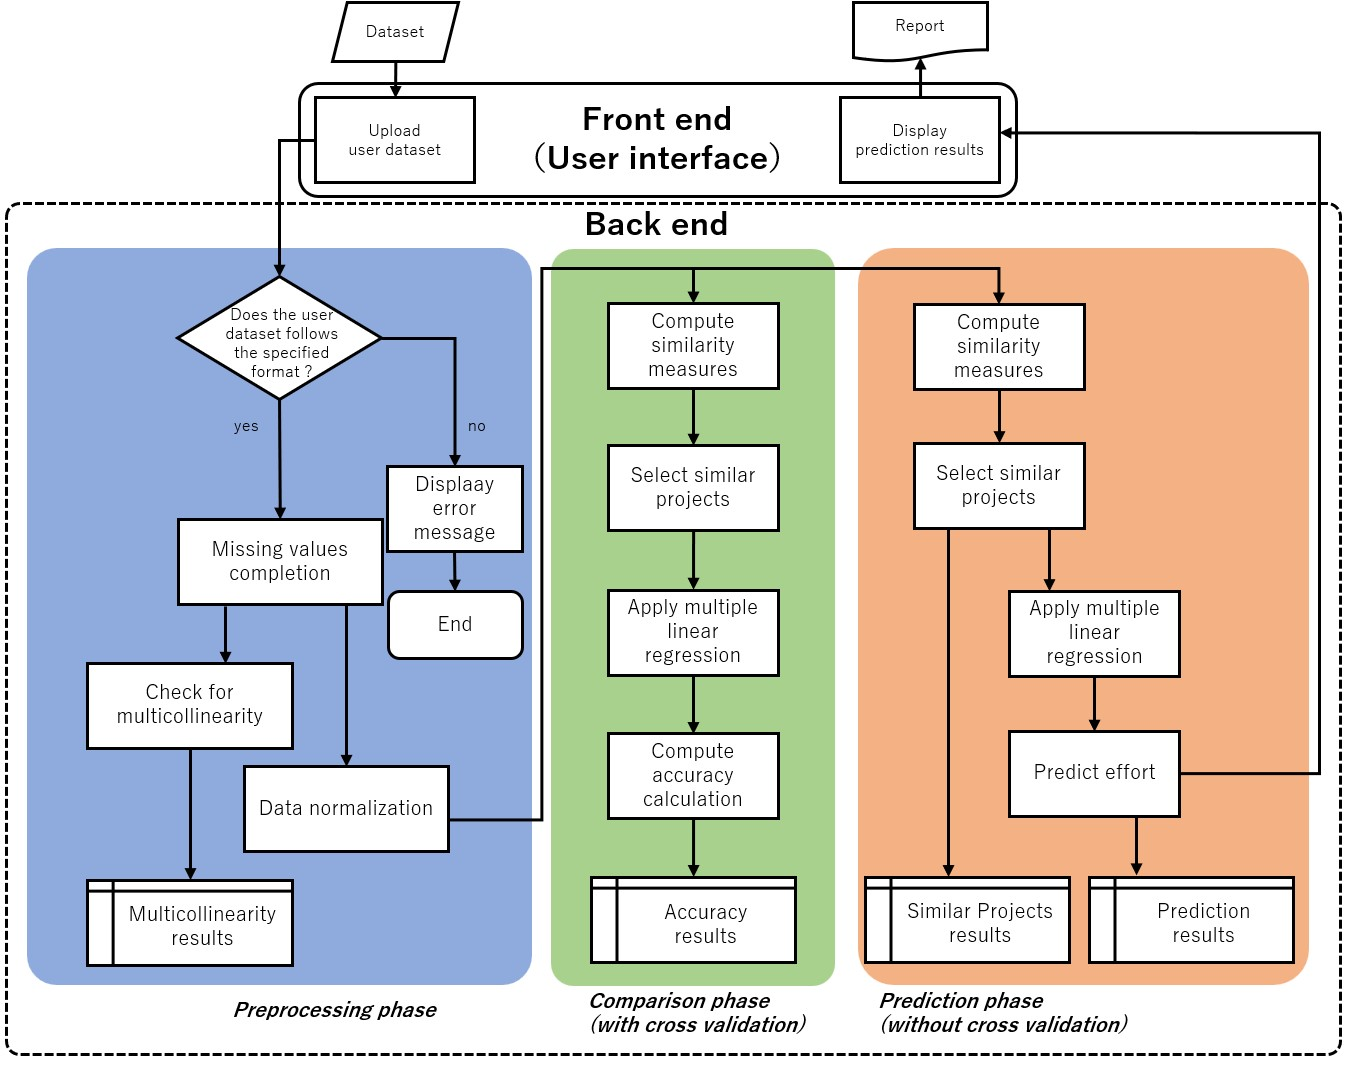
\includegraphics[width=120mm]{figure/fig/SystemArch_20241123.jpg}
  \captionsetup{labelformat=empty} % 図番号を非表示に設定
  \caption{\Fdualcaption{System Architecture of SDepT v2.0.0.}{SDepT v2.0.0 システム構成図.}}
  \label{fig:systemarch}
\end{figure}
% ラベルを英語にするのか日本語にするのか統一する

%%%%%%%%%%%%%%%%%%%%%%    3.1    %%%%%%%%%%%%%%%%%%%%%%
\clearpage
\subsection{フロントエンド}\label{subsec:3.1}
%フロントエンドの概要, 図も載せる予定
%現状フロントエンドの部分は去年と同じ
フロントエンドはHTML,CSS,Java Scriptを用いて実装している.
フロントエンドには2つのタブがあり,ユーザーは予備知識のレベルに応じて操作画面を選択することができる.
図\ref{fig:FrontBasic}および図\ref{fig:FrontAdvance}はそれぞれの操作画面であり,図\ref{fig:FrontBasic}はBasic画面,図\ref{fig:FrontAdvance}はAdvabce画面となっている.
1つ目のBasic画面では,ユーザーが精度と処理速度で重視する方を選択するのみで実行できるため,専門的な知識を必要としない.
一方,Advance画面では,ユーザーは各工程で用いる手法の選択が可能である.
さらに,類似プロジェクトの選定方法はそれぞれの$k$の値(それぞれの手法の類似プロジェクト選出範囲を調整できる(\ref{Selection}項参照))を選択できるため,より自由度の高い操作が可能となっている.手法を選択するため専門的な知識を要するが,選択した手法のみで実行できるため実行時間の短縮が期待できる.
どちらの画面においても,過去プロジェクトと新規プロジェクトのプロジェクト特性についてのデータセットをアップロードするが,必須項目は過去プロジェクトの開発工数のみである.
そのため,ユーザーが所有しているデータを最大限活用することができる.
予測結果は,csv形式のレポートとしてユーザーに返され,以下の項目が記載されている.
\begin{itemize}
  \item 各手法ごとの新規プロジェクトの開発工数予測値
  \item 各手法の予測精度
  \item 新規プロジェクトの類似プロジェクト
  \item VIF値
\end{itemize}

レポートを活用した開発工数の予測方法は,\ref{sec:4}で使用例を用いて解説する.
\begin{figure}[t]
  \centering
  % 左側の図
  \begin{minipage}[t]{0.49\textwidth}
      \centering
      \fbox{\includegraphics[width=0.9\textwidth]{figure/fig/Frontend_Basic.pdf}} % 左の画像
      \captionsetup{labelformat=empty} % 図番号を非表示に設定
      \caption{\Fdualcaption{“Basic” Tab of User interface.}{Basic画面のユーザインターフェース.}}
      \label{fig:FrontBasic}
  \end{minipage}
  \hfill
  % 右側の図
  \begin{minipage}[t]{0.49\textwidth}
      \centering
      \fbox{\includegraphics[width=0.9\textwidth]{figure/fig/Frontend_Advance.pdf}} % 右の画像
      \captionsetup{labelformat=empty} % 図番号を非表示に設定
      \caption{\Fdualcaption{“Advance” Tab of User interface.}{Advance画面のユーザインターフェース.}}
      \label{fig:FrontAdvance}
  \end{minipage}
\end{figure}
% コメント参照、ページのボトムに図を配置する

%%%%%%%%%%%%%%%%%%%%%%    3.2    %%%%%%%%%%%%%%%%%%%%%%
% 全部書いて見ないとわからないけど、次のページ行ってもいいかも
% \clearpage
\subsection{バックエンド}\label{subsec:3.2}
バックエンドはR言語を用いて実装している.
本節では,\ref{Preprocess}項で前処理,\ref{PastPrediction}項で複数工数予測手法の比較,\ref{NewPrediction}項で新規プロジェクトの工数予測の処理について詳しく述べる.
\subsubsection{前処理}\label{Preprocess}
%前処理について
前処理は主に4つの工程に分かれる.
\begin{enumerate}[label=前処理(\arabic*), leftmargin=6.0em]
  \item アップロードされたデータセットが以下の所定書式に沿っているか判定する.
  \begin{itemize}
    \item 1列目にプロジェクト番号が含まれているか.
    \item データセットの値が全て数値で入力されているか.
    \item 開発工数の列名が「Effort」となっているか.
    \item 新規プロジェクトのデータが最終行に格納されており目的変数がNULLとなっているか.
  \end{itemize}
  所定書式に沿っていない場合は操作画面にエラーメッセージが表示され,処理が終了する.
  \item データセットに欠損値が含まれていた場合,欠損値の補完をする.
  SDepT v2.0.0では欠損値の補完手法として,中央値補完,平均値補完,最頻値補完,$k$最近傍補完の4手法を採用している.(\ref{Imputation}項参照)
  \item 過去プロジェクトの説明変数間の多重共線性の有無を確認する.
  多重共線性とは,説明変数間で相関係数が高い組み合わせが存在することをいう.
  多重共線性が認められた場合,回帰係数が異常値になり回帰の精度に悪影響を及ぼす可能性がある.
  多重共線性は検出指標または分散拡大要因と呼ばれる VIF (Variance Inflation Factor) 値で判断できる.
  VIF値は式\ref{VIF}により算出する.
  \begin{equation}
    \label{VIF}
    VIF_{i}=  \frac{1}{(1 - R_{i}^{2} )}
  \end{equation}
  \begin{center}
  $i:$ 説明変数の個数$R_{i}:$ 回帰係数
  \end{center}
  $R_{i}^{2}$はVIFを求めたいデータセットの説明変数$x_{i}$を目的変数とし,その他の説明変数を説明変数として回帰した際の決定係数である.
  一般的にVIF \textgreater 10の場合に説明変数間に多重共線性があると判定を行う.
  これはVIF = 10であるなら相関係数に換算すると約 0.95 であり2変数の関連性が非常に強いことを意味するからである.
  \item 全ての特徴が同じ程度の影響度を持つように,データセットを正規化する.
  SDepT v2.0.0では正規化手法として,Huangら\cite{Huang2017}が比較していた3手法(Z-score,Min-Max[0,1],Min-Max[-1,1])に加え回帰分析によく使われる正規化手法の一つであるBox-Cox変換の計4手法を採用している.(\ref{Normalization}項参照 )
  以降の複数工数予測手法の比較や新規プロジェクトの工数予測は,ここで正規化されたデータを用いている.
  
\end{enumerate}
\subsubsection{複数工数予測手法の精度比較}\label{PastPrediction}
複数工数予測手法の精度比較では,ハイブリッド回帰ベースの予測アプローチ\cite{Hybrid}が実装されている.
主に4つの工程に分かれる.
\begin{itemize}
  \item 過去プロジェクト同士の類似度の計算
  \item 類似プロジェクトの選定
  \item 回帰による予測プロジェクトの算出
  \item 予測精度の比較
\end{itemize}
上記の各工程では,複数の手法が用意されており,それらの組み合わせによって計288種類の手法の提供が可能である.
各プロジェクトデータにおいて各手法における予測精度を算出することで,ユーザー側で比較が可能になる.
また,本工程では精度比較の際にleave-one-out cross validation法\cite{Kohavi1995}を実装している.
上記の工程は以下の手順で進む.
\begin{enumerate}[label=(\arabic*)]
  \item データセットの過去プロジェクトの中から1つ選択し、仮予測プロジェクトとする.
  \item 仮予測プロジェクトとそれ以外の過去プロジェクトの類似度を算出する.
  \item 算出した類似度を小さい順に並び替え,類似プロジェクトの選定手法によって選出された過去プロジェクトを類似プロジェクトとする.
  \item 選出した類似プロジェクトを元に8種類の回帰を適用し,仮予測プロジェクトの開発工数の予測値を算出する.
  \item 全ての過去プロジェクトに対して(1)~(4)を繰り返し行う.
  \item 上記の工程で算出された予測値を元に,各手法の予測精度を評価する.
\end{enumerate}
\subsubsection{新規プロジェクトの工数予測}\label{NewPrediction}
新規プロジェクトこ工数予測では,複数工数予測手法の比較で実装した288種類の手法を用いて,新規プロジェクト開発工数を予測する.

%%%%%%%%%%%%%%%%%%%%%%    3.3    %%%%%%%%%%%%%%%%%%%%%%
\clearpage
% 表はsection 3.3.1の上かな
\subsection{開発工数予測手法}\label{subsec:3.3}
\begin{table}[h]
  \centering
  \captionsetup{labelformat=empty} % 図番号を非表示に設定
  \caption{\Tdualcaption{Comparison of SDepT v1.0.0 and SDepT v2.0.0.}{SDepT v1.0.0とSDepT v2.0.0の比較.}}
  \label{table:Comparison}
    \begin{tabular}{|l|c|c|}
      \hline
      ~ & SDepT v1.0.0 & SDepT v2.0.0 \\ \hline
      %%%%%%%%正規化手法%%%%%%%%
      \multirow{4}{*}{欠損値補完手法} & 中央値補完 & 中央値補完 \\
       & & 平均値補完 \\
       & & 最頻値補完 \\
       & & $k$最近傍補完 \\ \hline
      %%%%%%%%欠損値補完手法%%%%%%%%
      \multirow{4}{*}{正規化手法} & z-score法 & z-score法 \\
       & & MinMax[0, 1] \\
       & & MinMax[-1, 1] \\
       & & BoxCox法 \\ \hline
      %%%%%%%%特徴選択手法%%%%%%%%
      \multirow{8}{*}{回帰手法} & OLS & OLS \\
       & Ridge & Ridge \\
       & Lasso & Lasso \\
       & Elastic Net & Elastic Net \\
       & SCAD & SCAD \\
       & MCP & MCP \\
       & & Adaptive Lasso \\
       & & Non-Negative Garrote \\ \hline
    \end{tabular}
\end{table}
本節では,本ツールで実装した前処理手法及びハイブリッド予測手法\cite{Hybrid}について説明する.本節では,\ref{Imputation}項では欠損値の補完手法,\ref{Normalization}項では正規化手法,\ref{Distance}項では類似度計算手法,\ref{Selection}項では類似プロジェクトの選定手法,\ref{Regression}項では回帰手法,\ref{Evaluation}項では評価尺度に用いた手法について紹介する.
なお,SDepT v2.0.0はSDepT v1.0.0と比べ,欠損値補完手法,正規化手法,回帰手法が拡張されており,変更点を表\ref{table:Comparison}に示す.
% 図じゃなくてtexで表で書いた方が見やすいかも

\subsubsection{欠損値補完手法}\label{Imputation}
欠損値補完手法には4つの手法を採用している.
\paragraph{中央値補完 \quad \\}
中央値補完はデータの中央値で欠損値を補完する手法である.
中央値は外れ値の影響を受けにくく,数値データに適している.
\paragraph{平均値補完 \quad \\}
平均値補完はデータの平均値で欠損値を補完する手法である.
外れ値が存在する場合,平均値は影響を受けやすいが,欠損値を全体の分布に近づけることができる.
\paragraph{最頻値補完 \quad \\}
最頻値補完はデータの最頻値で欠損値を補完する方法である.
カテゴリデータや離散的な数値データに適しており,データの分布を反映しやすい.
%SDepT v2.0.0では連続的な数値データの処理を想定しているため,あまり適さない可能性がある.
\paragraph{$k$最近傍補完 \quad \\}
$k$最近傍補完は,欠損値を含むプロジェクトにより近いk個のデータの平均値や中央値で欠損値を補完する方法である.
プロジェクト同士の距離を計算するため,大量のデータでは効率が悪くなってしまう場合があるが,データの分布やパターンを活かした高度な補完が可能である.
SDepT v2.0.0においては,$k=5$とし,数値データの場合は平均値,カテゴリデータの場合は最頻値で補完される.

\subsubsection{正規化及び標準化手法}\label{Normalization}
% 基本的に式の後にカンマ、句読点をつける (OR学会の添削でシャオ先生が式の後にカンマ、句読点をつけるように添削してたはず)
正規化手法には4つの手法を採用している.
\paragraph{Z-score法 \quad \\}
Z-score法\cite{Huang2017}は,平均$0$,分散$1$にデータを標準化する手法であり,式(\ref{Z-score})のように標準化される.
\begin{equation}
  \label{Z-score}
  x'_{i,j} = \frac{x_{i,j} - \bar(X_j)}{std(X_j)}.
\end{equation}
\begin{center}
  $x_{i,j}$:$i$番目のプロジェクトの$j$番目の説明変数,$X_j$:$j$列目のデータ列,$std(X_j)$:$X_j$の標準偏差
\end{center}

\paragraph{Min-Max$\lbrack0, 1\rbrack$ \quad \\}
Min-Max$\lbrack0, 1\rbrack$\cite{Huang2017}は,データを$0$から$1$の範囲に正規化する手法であり,式(\ref{MinMax01})のように正規化される.
\begin{equation}
  \label{MinMax01}
  x'_{i,j} = \frac{x_{i,j} - \min(X_j)}{\max(X_j) - \min(X_j)}
\end{equation}
\begin{center}
  $x_{i,j}$:$i$番目のプロジェクトの$j$番目の説明変数,$X_j$:$j$列目のデータ列
\end{center}

\paragraph{Min-Max$\lbrack-1, 1\rbrack$ \quad \\}
Min-Max$\lbrack-1, 1\rbrack$\cite{Huang2017}は,データを$-1$から$1$の範囲に正規化する手法であり,式(\ref{MinMax-11})のように正規化される.
\begin{equation}
  \label{MinMax-11}
  x'_{i,j} = 2 \cdot \frac{x_{i,j} - \min(X_j)}{\max(X_j) - \min(X_j)} - 1
\end{equation}
\begin{center}
  $x_{i,j}$:$i$番目のプロジェクトの$j$番目の説明変数,$X_j$:$j$列目のデータ列
\end{center}

\paragraph{BoxCox \quad \\}
BoxCox法は,式(\ref{BoxCox})のように正規化される.
\begin{equation}
  \label{BoxCox}
  x'_{i,j} = 
    \begin{cases} 
    \frac{x_{i,j}^\lambda - 1}{\lambda} & \text{if } \lambda \neq 0 \\
    \ln(x_{i,j}) & \text{if } \lambda = 0
    \end{cases}
\end{equation}
\begin{center}
  $x_{i,j}$:$i$番目のプロジェクトの$j$番目の説明変数,$\lambda$:BoxCox変換におけるパラメータ
\end{center}
BoxCox変換は$\lambda$の値によって以下のように変換の性質が変わる.
\begin{itemize}
  \item $\lambda=1$:元のデータを保持
  \item $\lambda=0$:対数変換($ln(x)$)
  \item $\lambda<1$:外れ値を抑える
  \item $\lambda>1$:データのばらつきを強調
\end{itemize}

\subsubsection{類似度計算手法}\label{Distance}
類似度計算には3つの手法を採用している.
\paragraph{ユークリッド距離(Euclidean Distance; ED) \quad \\}
% 参考文献の順番が若い番号順になるようにする。
ユークリッド距離\cite{Dejaeger2012}\cite{Shepperd1997}は,CBRで最も多く用いられている類似度尺度である.
予測プロジェクト$a$と過去プロジェクト$p$のユークリッド距離$ED_{a,p}$は式(\ref{ED})によって求める.
\begin{equation}
  \label{ED}
  ED_{a,p} = \sqrt{\sum_{j=1}^{n}(x'_{a,j} - x'_{p,j})^2}
\end{equation}
\paragraph{重み付きユークリッド距離(Weighted Euclidean Distance; W\_ED) \quad \\}
重み付きユークリッド距離は,通常のユークリッド距離における各プロジェクト特性の差にプロジェクト特性ごとに異なる重みをかけることで,特定のプロジェクト特性の重要度を付与することを可能にしている.
重み付きユークリッド距離を定式化したものが式(\ref{W_ED})である.
ここで,予測プロジェクトは$a$,過去プロジェクトは$p$,重み付きユークリッド距離は$wED$とする.
プロジェクト特性ごとの重み$w_i$は,菅\cite{菅2017}が紹介しているカテゴリースコアの算出法を採用している.
\begin{equation}
  \label{W_ED}
  wED_{a,p} = \sqrt{\sum_{j=1}^{n}w_i・(x'_{a,j} - x'_{p,j})^2}
\end{equation}
\paragraph{コサイン類似度(Cosine Similarity; COS) \quad \\}
コサイン類似度は,2つのベクトルのなす角のコサイン値を算出することで類似度を測定する手法である.
2つのベクトルの内積を2つのベクトルの大きさで割ることで計算される(\ref{COS}).
%値が$-1\sim1$に正規化されるため,正規化していない数値を式(\ref{COS})に代入し類似度を算出する.
\begin{equation}
  \label{COS}
  COS_{a,p}=\frac{\sum_{j=1}^{m}x'_{a,j}・x'_{p,j}}{\sqrt{\sum_{j=1}^{m}(x'_{a,j})^2}\sqrt{\sum_{j=1}^{m}(x'_{p,j})^2}}
\end{equation}
\subsubsection{類似プロジェクト選定手法}\label{Selection}
類似プロジェクト選定には3つの手法を採用している.
\paragraph{クラスタリング \quad \\}
クラスタリング\cite{Hai2022}は異なる性質のものが混ざり合った集団から,互いに似た性質を持つものを集め,クラスタ (集合) をつくる方法である. クラスタ分析には様々な手法があるが,本研究では,非階層型クラスタ分析手法の一つでありソフトウェア開発労力の予測にも用いられている,$k$-means法を採用する.
% 階層型クラスタ分析はあらかじめ分割するクラスタの数を決める必要がなく, 結果の全体像を樹形図に表示できるため, 全体に対するサンプルの位置づけ, 形成されたクラスタ間の相対的な位置づけが比較できる. 一方, 非階層型クラスタ分析では, あらかじめクラスタの数を指定する必要があり, 全体像の解釈は困難である. 階層型の短所としては対象を一度分類すると分類が確定してしまうため, 信頼性が低い. それに対して非階層型は一度分類してもそれより適した分類になるまでクラスタ間を移動させるため, より自然で信頼性の高い分類が可能になる. 一般的な非階層型クラスタ分析の手法として, k-means法が代表的であり, ソフトウェア開発労力の予測にも用いられている. そこで, 本研究はk-means法を用いる.
一般的に$k$-means法は, 次のようにクラスタを生成する.
% 手順なら(1), (2)てきな感じで書く(他の手順の説明がこの表記で書かれているみたいだから)
\begin{enumerate}
  \item クラスタの核 (クラスタの中心) を$k$個仮定する.
  \item 核の位置が変化しなくなるまで以下を繰り返す.
  \begin{itemize}
    \item 各プロジェクトを最も距離の短い核のクラスタに分類する.
    \item 各クラスタに分類されたプロジェクトの平均を該当クラスタの新しい核とする.
  \end{itemize}
\end{enumerate}
本研究では,予測プロジェクトが含まれるクラスタに分類された過去プロジェクトを類似ブロジェクトとして選出する.
また,クラスタの数$k$はユーザ自身で設定が可能であり,デフォルトでは$k=2,3,4,5$としている.
\paragraph{Fixed-$k$ \quad \\}
Fixed-$k$では昇順にソートした類似度の,小さいものから$k$個を類似プロジェクトとして選定する.
$k$の取り方はユーザ自身で設定が可能であり,デフォルトでは$k=3,4,5,6$となっている.
\paragraph{四分位数法 \quad \\}
四分位数法は,Fixed-$k$と同様に類似度を昇順にソートし,四等分することで類似プロジェクトを選定する手法である.
以下の手順によって選定を行う.
\begin{enumerate}[label=(\arabic*)]
  \item 予測プロジェクトとの類似度を昇順にソートする
  \item 昇順にした類似度ベクトルを四等分する
  \item 四等分したもののうち,より類似度の近い集合$k$個を類似プロジェクトとして選定する
\end{enumerate}
ここでの$k$もユーザ自身が設定でき,デフォルトは$k=1,2,3,4$である.
分割パターンは全てFixed-$k$の分割パターンに含まれているが,全体に対して類似プロジェクトとして選定されている割合がイメージしやすいため採用している.
\subsubsection{回帰手法}\label{Regression}
一般的に,線形重回帰モデルは式(\ref{LMR})で表される.
\begin{equation}
  \label{LMR}
  Y_{i} = \sum_{j=0}^{n}{\beta_{j}X_{i,j}+\epsilon}
\end{equation}
ここで,$Y_{i}$と$X_{i,j}$はそれぞれ,プロジェクト$i~(i=1,~2,...,~m)$の開発工数とプロジェクト特性$j~(i=1,~2,...,~n)$を表す.また,$\beta_0,~\beta_1,~...,~\beta_n$は回帰係数であり,$\epsilon$は確率誤差項である.
正規化済みデータを用いて回帰を行い,回帰の後逆変換を施すことで予測値を算出する.
% このモデルは,誤差の平均が0,分散が一定であるという仮定の元に成り立つため,回帰を行う前に対数変換を行う.回帰ののちに逆対数変換の処理を施すことで予測値を算出する.
% また,回帰を行う前に対数変換を行い,回帰後の値に逆対数変換の処理を施すことで予測値を算出する.
%線形重回帰モデルを用いる際に,以下の4つの仮定を設ける.
%\begin{enumerate}[(仮定1)]
  %\item 誤差の平均値が0である. \\ $E[\epsilon]=0.$
  %\item 誤差の分散が一定である. \\ $Var[\epsilon]=\sigma^2.$
  %\item 各誤差は互いに独立であり,その共分散は0である. \\ $E[\epsilon_i \epsilon_i']=0, (i\neq i',~i=1,~2,~...,~m,~i'=1,~2,~...,~m)$
  %\item 誤差は以下のような正規確率密度関数に従う. \\ $p(z)=(2\pi\sigma^2)^(-1/2)\exp[z^2/2\sigma^2]$
%\end{enumerate}
%これらの仮定を満たすために回帰を行う前に対数変換を行い,回帰ののち逆対数変換の処理を施すことで予測値を算出する.
回帰には8つの手法を採用している.

\paragraph{最小二乗法(Ordinary Least Squares; OLS) \quad \\}
回帰係数を$\beta(\beta=\beta_0,\beta_1,...,\beta_m)$とし,OLSによる推定値$\hat{\beta}_{OLS}$は式(\ref{OLS})によって与えられる.
\begin{equation}
  \label{OLS}
  \bm{\hat{\beta}}_{OLS} = \underset{\bm{\beta}}{\arg min}\sum_{i=1}^{n}(y_{i} -\sum_{j=0}^{m}\beta_{j}x_{i,j})^2
\end{equation}
%ここで,説明変数には互いに強い相関を持つことが多く,多重共線性が存在する場合においてはOLSでの推定値が不安定になることが知られている.
%対策として,説明変数の選択を行うことが効果的である.
%目的変数に対して効果的である説明変数を残すために,本研究ではステップワイズ法を採用する.
%また,変数選択の評価尺度には赤池情報量基準(Akaike Infomation Criterion;AIC)\cite{AIC}を用いる.

\paragraph{Ridge回帰 \quad \\}
Ridge回帰\cite{Ridge}\cite{Araki2013}\cite{Hastie2009}は,罰則項がついている回帰手法である.
罰則項により,多重共線性に対処できる.
式(\ref{Ridge})によって算出され,式中の$\lambda\sum_{j=1}^{m}\beta_{j}^2$が罰則項である.
$\lambda$によって罰則項の強さが調整でき,$\lambda=0$のときOLSとなり,$\lambda$が大きいほど罰則が強くなる.
%また,Ridge回帰と後述のLasso回帰の制約領域の模式図を図\ref{fig:ridge_lasso}に示す.
\begin{equation}
  \label{Ridge}
  \bm{\hat{\beta}_{Ridge}} =\underset{\bm{\beta}}{\arg min}\lbrace\sum_{i=1}^{n}(y_{i} -\sum_{j=0}^{m}\beta_{j}x_{i,j})^2 +\lambda\sum_{j=1}^{m}\beta_{j}^2\rbrace
\end{equation}
%% \begin{figure}[h]
%   \centering
%   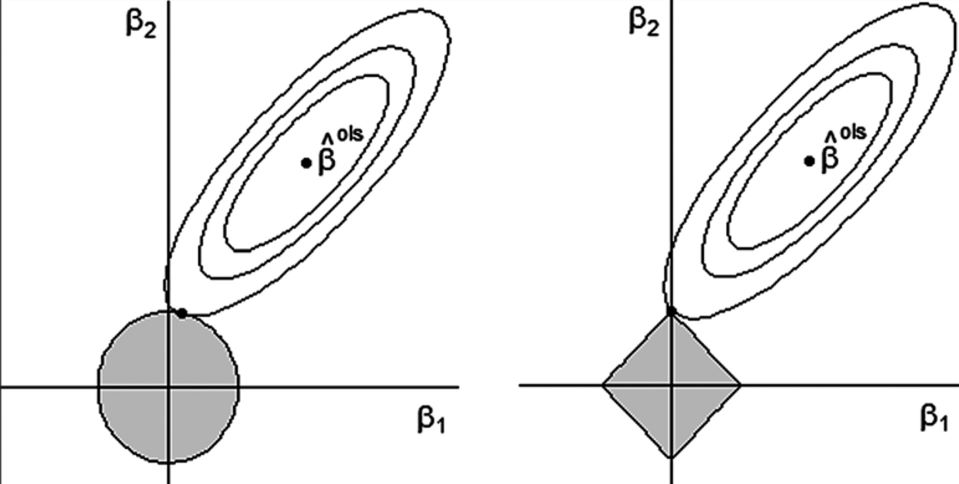
\includegraphics[width=120mm]{figures/fig/ridgelasso.jpg}
%   \caption{Ridge回帰とLasso回帰の制約領域の模式図\cite{RidgeLasso2}}
%   \label{fig:ridge_lasso}
% \end{figure}

\paragraph{Lasso回帰 \quad \\}
Lasso回帰\cite{Araki2013}\cite{Hastie2009}\cite{Tibshirani2018}は,Ridge回帰と同様,罰則項がついている回帰手法である.
Lasso回帰は式(\ref{Lasso})で算出される.
Ridge回帰と異なる点は,罰則項が$\lambda\sum_{j=1}^{m}|\beta_{j}|$となっている点である.
\begin{equation}
  \label{Lasso}
  \bm{\hat{\beta}_{Lasso}} =
\underset{\bm{\beta}}{\arg min}\lbrace\sum_{i=1}^{n}(y_{i} -\sum_{j=0}^{m}\beta_{j}x_{i,j})^2 +\lambda\sum_{j=1}^{m}|\beta_{j}|\rbrace
\end{equation}
\vskip\baselineskip

\paragraph{Elastic Net回帰 \quad \\}
ElasticNet回帰\cite{Zou2005}は,Ridge回帰とLasso回帰の罰則項をどちらも採用している回帰手法である.
式(\ref{Elastic})によって算出される.
\begin{equation}
  \label{Elastic}
  \bm{\hat{\beta}_{Elastic}} =
\underset{\bm{\beta}}{\arg min}\lbrace\sum_{i=1}^{n}(y_{i} -\sum_{j=0}^{m}\beta_{j}x_{i,j})^2 +\lambda\sum_{j=1}^{m}(\frac{1}{2}(1-\alpha)\beta_{j}^2+\alpha|\beta_{j}|)\rbrace
\end{equation}
\paragraph{SCAD回帰 \quad \\}
SCAD回帰\cite{Fan2001}は,Lasso回帰の拡張として提案された回帰手法である.
大きな係数に対してはLasso回帰,小さな係数に対してはRidge回帰の罰則項のような効果を持つという特徴がある.
式(\ref{SCAD})で算出でき,罰則項は式(\ref{SCAD_J})で与えられる.
\begin{equation}
  \label{SCAD}
  \bm{\hat{\beta}_{SCAD}} =\underset{\bm{\beta}}{\arg min}\lbrace\frac{1}{2}\sum_{i=1}^{n}(y_{i} -\sum_{j=0}^{m}\beta_{j}x_{i,j})^2 +\sum_{j=1}^{m}J(\beta_{j})\rbrace
\end{equation}
\begin{equation}
  \label{SCAD_J}
  J(\beta)=
  \begin{cases}
    \lambda|\beta| &(|\beta|\le\lambda) \\
    \frac{\beta^2-2a\lambda|\beta|+\lambda^2}{2(a-1)} &(\lambda<|\beta|\le a\lambda) \\
    \frac{(a+1)\lambda^2}{2} &(|\beta|>a\lambda)
  \end{cases}
\end{equation}
\paragraph{MCP回帰 \quad \\}
MCP (Multiple Change Points;MCP)回帰\cite{Zhang2010}は,SCAD回帰同様,Lasso回帰の拡張として提案された回帰手法である.
SCAD回帰よりも構造が簡単で,計算が容易であるという利点を持つ.
式(\ref{MCP})で算出でき,罰則項は式(\ref{MCP_J})で与えられる.
\begin{equation}
  \label{MCP}
  \bm{\hat{\beta}_{SCAD}} =\underset{\bm{\beta}}{\arg min}\lbrace\frac{1}{2}\sum_{i=1}^{n}(y_{i} -\sum_{j=0}^{m}\beta_{j}x_{i,j})^2 +\sum_{j=1}^{m}J(\beta_{j})\rbrace
\end{equation}
\begin{equation}
  \label{MCP_J}
  J(\beta)=
  \begin{cases}
    \lambda|\beta|-\frac{x^2}{2a} &(|\beta|\le a\lambda) \\
    \frac{a\lambda^2}{2} &(|\beta|>a\lambda)
  \end{cases}
\end{equation}

\paragraph{Adaptive Lasso回帰 \quad \\}
AdaptiveLasso回帰\cite{Zou2006}\cite{Araki2013}は2段階推定を行う回帰手法である.
第1段階で$\bm{\beta}$の初期推定量(本研究では$\bm{\hat{\beta}}_{ridge}$)を求め,第2段階で,式(\ref{AdaptiveWeight})を用いて算出した重み$\hat{\omega}_{j}$をペナルティとして課した罰則項付き回帰(式(\ref{AdaptiveLasso}))を行う.
なお,本研究では$\gamma=2$とした.
\begin{equation}
  \label{AdaptiveWeight}
  \hat{\omega}_{j}= 
  \begin{cases} 
  \frac{1}{|\bm{\beta}_{ridge.j}|^\gamma} & \text{where } \bm{\beta}_{ridge.j} \neq 0\\
  \inf & \text{where } \bm{\beta}_{ridge.j} = 0
  \end{cases}
\end{equation}
\begin{equation}
  \label{AdaptiveLasso}
  \bm{\hat{\beta}_{AdaptiveLasso}} =
\underset{\bm{\beta}}{\arg min}\lbrace\sum_{i=1}^{n}(y_{i} -\sum_{j=0}^{m}\beta_{j}x_{i,j})^2 +\lambda\sum_{j=1}^{m}\hat\omega_{j}|\beta_{j}|\rbrace
\end{equation}

\paragraph{Non-Negative Garrote回帰 \quad \\}
Non-NegativeGarrote回帰\cite{Zou2006}\cite{Araki2013}は,非負の因子である$c=(c_{1}, c_{2},\dots,c_m)$を用いて$\bm{\hat{\beta}}$の要素を直接縮小して推定する手法である.式(\ref{NonNegativeGarrote})で与えられる.
\begin{equation}
  \label{NonNegativeGarrote}
  \begin{split} 
  \bm{\hat{\beta}_{NonNegative}} =
  &\underset{\bm{\beta}}{\arg min}\lbrace\sum_{i=1}^{n}(y_{i} -\sum_{j=0}^{m}\bm{\beta}_{ols.j}x_{i,j}c_{j})^2 +\lambda\sum_{j=1}^{m}|c_{j}|\rbrace\\
  &c_{j}\geq0
  \end{split} 
\end{equation}

\subsubsection{評価尺度}\label{Evaluation}
評価尺度には4つの手法を採用している.
\paragraph{MMRE(Mean Magnitude of Relative Error) \quad \\}
MMREとはMREの平均値であり,MREは予測値と実測値との相対誤差を表す指標である.
プロジェクト$i$の開発工数値$y_{i}$と予測値$\hat{y_{i}}$の$MRE_{i}$は式(\ref{MRE})によって算出され,$MMRE$は式(\ref{MMRE})によって算出される.
数値が小さいほど予測精度が高いことを示す.
\begin{equation}
  \label{MRE}
  MRE_{i} = \frac{|y_{i}-\hat{y}_{i}|}{y_{i}}
\end{equation}
\begin{equation}
  \label{MMRE}
  MMRE = \frac{\sum_{i=1}^{n}MRE_{i}}{n}
\end{equation}
\paragraph{MdMRE(Median Magnitude of Relative Error) \quad \\}
MdMREはMREの中央値である.
MdMREはMREと同様に数値が小さいほど予測精度が高いことを示す.
\paragraph{Pred($p$) \quad \\}
Pred($p$)\cite{Port2008}は予測値と実測値のMREが$p$\%以下となった割合を示し,数値が大きいほど予測精度が高いことを示す.
本実験では,Pred($25$)と設定して開発を行う.
MREが25\%以下となったプロジェクトの件数を$s$と置くとPred($25$)は式(\ref{Pred})にて算出される.
\begin{equation}
  \label{Pred}
  Pred(25) = 100 \times \frac{s}{n}
\end{equation}
\paragraph{SA(Standardized Accuracy) \quad \\}
SA\cite{Shepperd2012}は,Predと同様に数値が大きいほど予測精度が高いことを示し,式(\ref{SA})で算出される.
また,$MAE$は$i$番目のプロジェクトの実測工数$y_i$とその予測値$\hat{y_i}$との誤差平均であり,式(\ref{MAE})で算出される.
$MAE_{0}$は$\hat{y}$の代わりに,$j$番目のプロジェクトの実測工数$y_j$をランダムに割り当てた場合の絶対誤差平均であり,式(\ref{MAE0})で算出される.
\begin{equation}
  \label{SA}
  SA =\Big(1 - \frac{MAE}{MAE_{p0}} \Big) \times 100
\end{equation}

\begin{equation}
  \label{MAE}
  MAE =\frac{1}{m} \sum_{i=1}^{m} |y_{i} - {\hat{y}_{i}}|
\end{equation}

\begin{equation}
  \label{MAE0}
  MAE_{p0} =\frac{2}{m^2} \sum_{i=1}^{m} \sum_{j=1}^{j<i} |y_{i} - y_{j}|
\end{equation}


% 第4章
\clearpage
\pagestyle{plain}
\section{システム使用例}\label{sec:4}%%%システム使用例じゃなくてテストという単語を入れてもいいかも
%\ref{sec:4}では実際にシステムを動かした際の詳細を書く\par
% プロジェクト特性は箇条書きの方がいいかも
本章では、Desharnaisデータセット\cite{Desharnais89}を用いたSDepT v2.0.0のシステム使用例を示す.
Desharnaisデータセットは1980年代のカナダのソフトウェア開発会社のプロジェクトデータが記録されており,81件の過去のプロジェクトデータと11のプロジェクト特性(チームの経験年数(TeamExp in years),開発年度(YearEnd),マネージャーの経験年数(ManageExp in years),開発年数(Length),トランザクション数(Transactions),エンティティ数(Entities),調整済みファンクションポイント(PointsAdjust),調整係数(Envergure),未調整ファンクションポイント(PointsNonAdjust),開発言語(Language),開発工数(Effort))が含まれている.表\ref{table:DesharnaisDataset}にDesharnais データセットの一部を示す。
\begin{table*}[ht]
  \centering
  \captionsetup{labelformat=empty} % 図番号を非表示に設定
  \caption{\Tdualcaption{A Sample Dataset of Software Development.}{Desharnaisデータセット.}}
  \label{table:DesharnaisDataset}
  \begin{center}
    \resizebox{\textwidth}{!}{
      \begin{tabular}{|c|c|c|c|c|c|c|c|c|c|c|c|}
        \hline
        Project & TeamExp & ManagerExp & YearEnd & Length & Transactions & Entities & PointsAdjust & Envergure & PointsNonAjust & Language & Effort \\ \hline \hline
        1 & 1 & 4 & 85 & 12 & 253 & 52 & 305 & 34 & 302 & 1 & 5152 \\ \hline
        2 & 0 & 0 & 86 & 4 & 197 & 124 & 321 & 33 & 315 & 1 & 5635 \\ \hline
        3 & 4 & 4 & 85 & 1 & 40 & 60 & 100 & 18 & 83 & 1 & 805 \\ \hline
        \vdots & \vdots & \vdots & \vdots & \vdots & \vdots & \vdots & \vdots & \vdots & \vdots & \vdots & \vdots \\ \hline
        80 & 4 & 3 & 86 & 12 & 469 & 176 & 645 & 43 & 697 & 3 & 5880 \\ \hline
        81 & 4 & 4 & 85 & 36 & 886 & 241 & 1127 & 34 & 1116 & 1 & 23940 \\ \hline
      \end{tabular}
    }
  \end{center}
\end{table*}


% \begin{table}[h]
%   \centering
%   \caption{Desharnaisデータの特性一覧}
%   \label{table:Desh}
%   \begin{tabular}{|c|c|} \hline
%     チームの経験年数(TeamExp in years) & 開発年度(YearEnd) \\ \hline
%     マネージャーの経験年数(ManageExp in years) & 開発年数(Length) \\ \hline
%     トランザクション数(Transactions) & エンティティ数(Entities) \\ \hline
%     調整済みファンクションポイント(PointsAdjust) & 調整係数(Envergure) \\ \hline
%     未調整ファンクションポイント(PointsNonAdjust) & 開発言語(Language) \\ \hline
%     開発工数(Effort) & ~ \\ \hline
%   \end{tabular}
% \end{table}

\subsection{ユーザーインターフェース}
ユーザーは以下の手順で操作を行う.
\begin{enumerate}
  \item 「Upload」ボタンを押し,ユーザーデータセットをアップロードする.
  このとき,アップロードしたデータセットのファイル名が「Upload」ボタンの横に表示されていれば,正常にアップロードされている.
  また,データセットがアップロードされていない場合はサンプルデータセットとして「sampleData.csv」が使用される.
  \item \begin{itemize}
    % ここだけ箇条書きなの気持ち悪いかも
    % basic画面の場合 ~、advance画面の場合 ~ という風に書いた方がいいかも
    \item Basic画面では,予測精度を優先するか,計算速度を優先するかを選択できる.
    \item Advance画面では,各工程における採用手法を選択することができる.類似プロジェクト選定手法については,クラスタリングにおけるクラスタ数$k$,Fixed-kにおける選択プロジェクト数$k$,四分位数法における選択集合数$k$をそれぞれ任意に設定することができ,設定しなかった場合はデフォルトの数値で予測が行われる.
    \end{itemize}
  \item 「Predict」ボタンを押すことで予測が始まる.
  \item 計算が終了し画面が切り替わると,「Download」ボタンを押して予測結果をcsv形式でダウンロードすることができる.

% ここでbasicとadvanceをもう一度乗せてもいいかも

\end{enumerate}

\subsection{予測結果レポート}
開発工数の予測が完了すると,予測結果として新規プロジェクトの工数予測値,各手法の予測精度,新規プロジェクトに対する類似プロジェクト,VIF値がそれぞれcsvファイルとして返される.
実際には,前処理の組み合わせごとに最大16組(欠損値補完4手法$\times$正規化4手法)のレポートが返されるが,ここでは例として,中央値による欠損値補完及びZ-score正規化を施したデータの出力レポートを表\ref{table:est}~表\ref{table:vif}に示す.

\begin{table*}[ht]
  \centering
  \captionsetup{labelformat=empty} % 図番号を非表示に設定
  \caption{\Tdualcaption{``Predicted Effort for New Project" Report.}{新規プロジェクトの工数予測値.}}
  \label{table:est}
  \resizebox{\textwidth}{!}{
    \begin{tabular}{|l|r|r|r|r|r|r|r|r|}
      \hline
        ~ & OLS & Ridge & Lasso & ElasticNet & SCAD & MCP & AdaptiveLasso & NonNegativeGarrote \\ \hline
        ED-Clustering($k$=2) & 32084  & 14345  & 11868  & 12046  & 13481  & 13610  & 10924  & 19878  \\ \hline
        ED-Clustering($k$=3) & 10710  & 7149  & 28993  & 27931  & 3859  & 30606  & 19180  & 20900  \\ \hline
        ED-Clustering($k$=4) & -12352  & 5199  & 17626  & 15766  & 3399  & 3399  & 14332  & 17095  \\ \hline
        ED-Clustering($k$=5) & -12352  & 5199  & 17626  & 15766  & 3399  & 3399  & 14332  & 17095  \\ \hline
        ED-Fixed\_$k$($k$=3) & -6511  & 7132  & 4335  & 11471  & 4736  & 4717  & 6271  & 6513  \\ \hline
        ED-Fixed\_$k$($k$=4) & -23068  & 6749  & 7903  & 11635  & 4253  & 4253  & 7388  & -36596  \\ \hline
        ED-Fixed\_$k$($k$=5) & -19520  & 4536  & 9791  & 9921  & -33173  & -24506  & 4618  & -30628  \\ \hline
        ED-Fixed\_$k$($k$=6) & 16540  & 3241  & 17129  & 18240  & 3208  & 3208  & 9999  & 7079  \\ \hline
        ED-Quantile($k$=1) & 16236  & 13695  & 15497  & 15166  & 12976  & 14833  & 14485  & 16630  \\ \hline
        ED-Quantile($k$=2) & 18828  & 15615  & 15430  & 15001  & 15503  & 15376  & 15342  & 18105  \\ \hline
        ED-Quantile($k$=3) & 16336  & 14498  & 14649  & 13856  & 14669  & 18479  & 15563  & 16711  \\ \hline
        ED-Quantile($k$=4) & 16691  & 15753  & 16601  & 16482  & 16740  & 16740  & 16294  & 16798  \\ \hline
        WED-Clustering($k$=2) & 32084  & 14345  & 11868  & 12046  & 13481  & 13610  & 10924  & 19878  \\ \hline
        WED-Clustering($k$=3) & 10710  & 7149  & 28993  & 27931  & 3859  & 30606  & 19180  & 20900  \\ \hline
        WED-Clustering($k$=4) & -12352  & 5199  & 17626  & 15766  & 3399  & 3399  & 14332  & 17095  \\ \hline
        WED-Clustering($k$=5) & -12352  & 5199  & 17626  & 15766  & 3399  & 3399  & 14332  & 17095  \\ \hline
        WED-Fixed\_$k$($k$=3) & 805  & 1837  & 1836  & 1836  & 2400  & 1836  & 1836  & 1836  \\ \hline
        WED-Fixed\_$k$($k$=4) & 8053  & 1853  & 1760  & 1691  & 1778  & 1778  & 1737  & 1560  \\ \hline
        WED-Fixed\_$k$($k$=5) & 7285  & 1646  & 3005  & 2331  & 1669  & 1590  & 1374  & 1347  \\ \hline
        WED-Fixed\_$k$($k$=6) & 22665  & 1590  & 1537  & 1838  & 1537  & 1537  & 1537  & 31924  \\ \hline
        WED-Quantile($k$=1) & 14263  & 6230  & 2025  & 2030  & 8781  & 6853  & 2090  & 4292  \\ \hline
        WED-Quantile($k$=2) & 20305  & 14227  & 13056  & 13009  & 15503  & 15519  & 16405  & 18121  \\ \hline
        WED-Quantile($k$=3) & 19717  & 14509  & 17300  & 16788  & 17885  & 17922  & 17586  & 19787  \\ \hline
        WED-Quantile($k$=4) & 16691  & 15753  & 16601  & 16482  & 16740  & 16740  & 16294  & 16798  \\ \hline
        COS-Clustering($k$=2) & 32084  & 14345  & 11868  & 12046  & 13481  & 13610  & 10924  & 19878  \\ \hline
        COS-Clustering($k$=3) & 10710  & 7149  & 28993  & 27931  & 3859  & 30606  & 19180  & 20900  \\ \hline
        COS-Clustering($k$=4) & -12352  & 5199  & 17626  & 15766  & 3399  & 3399  & 14332  & 17095  \\ \hline
        COS-Clustering($k$=5) & -12352  & 5199  & 17626  & 15766  & 3399  & 3399  & 14332  & 17095  \\ \hline
        COS-Fixed\_$k$($k$=3) & 6941  & 10824  & 9460  & 9590  & 8690  & 8156  & 9434  & 9359  \\ \hline
        COS-Fixed\_$k$($k$=4) & 42787  & 8354  & 8708  & 7929  & 8708  & 8708  & 5624  & 18217  \\ \hline
        COS-Fixed\_$k$($k$=5) & 25354  & 8215  & 5170  & 3609  & 9906  & 7574  & 4480  & 14964  \\ \hline
        COS-Fixed\_$k$($k$=6) & -2326  & 7687  & 9281  & 9281  & 9281  & 9281  & -2385  & -2820  \\ \hline
        COS-Quantile($k$=1) & 15688  & 12392  & 13600  & 13090  & 15836  & 15940  & 14776  & 14475  \\ \hline
        COS-Quantile($k$=2) & 15997  & 15554  & 15608  & 15616  & 15538  & 15538  & 15852  & 16439  \\ \hline
        COS-Quantile($k$=3) & 16192  & 15527  & 15790  & 15741  & 15296  & 15296  & 12993  & 16221  \\ \hline
        COS-Quantile($k$=4) & 16691  & 15753  & 16601  & 16482  & 16740  & 16740  & 16294  & 16798  \\ \hline
    \end{tabular}
  }
\end{table*}

\begin{table*}[ht]
  \centering
  \captionsetup{labelformat=empty} % 図番号を非表示に設定
  \caption{\Tdualcaption{``Prediction Accuracy" Report (Partial).}{各手法の予測精度(一部抜粋).}}
  \label{table:eval}
  \begin{tabular}{|l|r|r|r|r|}
      \hline
        ~ & MMRE & MdMRE & Pred & SA \\ \hline
        ED-Clustering($k$=2)-OLS & 0.0314  & 0.3723  & 37.50  & 36.13 \\ \hline
        ED-Clustering($k$=2)-Ridge & 0.0050  & 0.3716  & 36.25  & 47.38 \\ \hline
        ED-Clustering($k$=2)-Lasso & 0.0296  & 0.3498  & 36.25  & 38.44 \\ \hline
        ED-Clustering($k$=2)-ElasticNet & 0.0300  & 0.3526  & 37.50  & 38.83 \\ \hline
        ED-Clustering($k$=2)-SCAD & 0.0317  & 0.3947  & 35.00  & 34.82 \\ \hline
        ED-Clustering($k$=2)-MCP & 0.0317  & 0.3904  & 35.00  & 36.80 \\ \hline
        ED-Clustering($k$=2)-AdaptiveLasso & 0.0252  & 0.3871  & 32.50  & 37.77 \\ \hline
        ED-Clustering($k$=2)-NonNegativeGarrote & 0.0273  & 0.3499  & 42.50  & 39.77 \\ \hline
        ED-Clustering($k$=3)-OLS & 0.0273  & 0.4461  & 27.50  & 0.90 \\ \hline
        \vdots & \vdots & \vdots & \vdots & \vdots  \\ \hline
        ED-Clustering($k$=3)-NonNegativeGarrote & 0.0120  & 0.3707  & 35.00  & 45.60 \\ \hline
        ED-Clustering($k$=4)-OLS & 0.0175  & 0.6129  & 31.25  & -14.20 \\ \hline
        \vdots & \vdots & \vdots & \vdots & \vdots  \\ \hline
        ED-Clustering($k$=5)-OLS & 0.0087  & 0.8410  & 23.75  & -61.35 \\ \hline
        \vdots & \vdots & \vdots & \vdots & \vdots  \\ \hline
        ED-Fixed\_$k$($k$=3)-OLS & 0.0102  & 0.8876  & 12.50  & -48.16 \\ \hline
        \vdots & \vdots & \vdots & \vdots & \vdots  \\ \hline
        ED-Fixed\_$k$($k$=6)-NonNegativeGarrote & 0.0139  & 0.5824  & 22.50  & 8.51 \\ \hline
        ED-Quantile($k$=1)-OLS & 0.0076  & 0.5452  & 28.75  & 28.91 \\ \hline
        \vdots & \vdots & \vdots & \vdots & \vdots  \\ \hline
        ED-Quantile($k$=4)-NonNegativeGarrote & 0.0039  & 0.3231  & 33.75  & 48.94 \\ \hline
        WED-Clustering($k$=2)-OLS & 0.0314  & 0.3723  & 37.50  & 36.13 \\ \hline
        \vdots & \vdots & \vdots & \vdots & \vdots  \\ \hline
        WED-Quantile($k$=4)-NonNegativeGarrote & 0.0039  & 0.3231  & 33.75  & 48.94 \\ \hline
        COS-Clustering($k$=2)-OLS & 0.0314  & 0.3723  & 37.50  & 36.13 \\ \hline
        \vdots & \vdots & \vdots & \vdots & \vdots  \\ \hline
        COS-Quantile($k$=4)-NonNegativeGarrote & 0.0039  & 0.3231  & 33.75  & 48.94 \\ \hline
        Analogy-based approach & \multirow{2}{*}{0.0025} & \multirow{2}{*}{0.5918} & \multirow{2}{*}{18.75} & \multirow{2}{*}{12.36} \\
        ED-Fixed$k$($k$=3)-Mean &  &  &  &  \\ \hline
  \end{tabular}
\end{table*}

\begin{table*}[ht]
  \centering
  \captionsetup{labelformat=empty} % 図番号を非表示に設定
  \caption{\Tdualcaption{``Similar Projects" report.}{新規プロジェクトの類似プロジェクトデータセット(一部抜粋).}}
  \label{table:sim}
  \resizebox{\textwidth}{!}{
    \begin{tabular}{|l|c|c|c|c|c|c|c|c|c|c|c|c|c|c|c|c|c|c|}
      \hline
      ~ & V1 & V2 & V3 & V4 & V5 & V6 & \dots & V9 & \dots & V16 & \dots & V20 & \dots & V40 & \dots & V60 & \dots & V80 \\ \hline
      ED-Clustering($k$=2) & 21 & 23 & 24 & 28 & 30 & 40 & \dots & 44 & \dots & 80 & ~ & ~ & ~ & ~ & ~ & ~ & ~ & ~ \\ \hline
      ED-Clustering($k$=3) & 21 & 40 & 42 & 44 & 67 & 73 & \dots & 80 & ~ & ~ & ~ & ~ & ~ & ~ & ~ & ~ & ~ & ~ \\ \hline
      ED-Clustering($k$=4) & 42 & 44 & 73 & 76 & 79 & 80 & ~ & ~ & ~ & ~ & ~ & ~ & ~ & ~ & ~ & ~ & ~ & ~ \\ \hline
      ED-Clustering($k$=5) & 42 & 44 & 73 & 76 & 79 & 80 & ~ & ~ & ~ & ~ & ~ & ~ & ~ & ~ & ~ & ~ & ~ & ~ \\ \hline
      ED-Fixed\_$k$($k$=3) & 38 & 50 & 68 & ~ & ~ & ~ & ~ & ~ & ~ & ~ & ~ & ~ & ~ & ~ & ~ & ~ & ~ & ~ \\ \hline
      ED-Fixed\_$k$($k$=4) & 38 & 47 & 50 & 68 & ~ & ~ & ~ & ~ & ~ & ~ & ~ & ~ & ~ & ~ & ~ & ~ & ~ & ~ \\ \hline
      ED-Fixed\_$k$($k$=5) & 37 & 38 & 47 & 50 & 68 & ~ & ~ & ~ & ~ & ~ & ~ & ~ & ~ & ~ & ~ & ~ & ~ & ~ \\ \hline
      ED-Fixed\_$k$($k$=6) & 3 & 37 & 38 & 47 & 50 & 68 & ~ & ~ & ~ & ~ & ~ & ~ & ~ & ~ & ~ & ~ & ~ & ~ \\ \hline
      ED-Quantile($k$=1) & 3 & 4 & 5 & 7 & 15 & 16 & \dots & 37 & \dots & 68 & \dots & 78 & ~ & ~ & ~ & ~ & ~ & ~ \\ \hline
      ED-Quantile($k$=2) & 3 & 4 & 5 & 7 & 8 & 10 & \dots & 16 & \dots & 29 & \dots & 40 & \dots & 78 & ~ & ~ & ~ & ~ \\ \hline
      ED-Quantile($k$=3) & 3 & 4 & 5 & 7 & 8 & 10 & \dots & 15 & \dots & 22 & \dots & 28 & \dots & 54 & \dots & 79 & ~ & ~ \\ \hline
      ED-Quantile($k$=4) & 1 & 2 & 3 & 4 & 5 & 6 & \dots & 9 & \dots & 16 & \dots & 20 & \dots & 40 & \dots & 60 & \dots & 80 \\ \hline
      WED-Clustering($k$=2) & 21 & 23 & 24 & 28 & 30 & 40 & \dots & 44 & \dots & 80 & ~ & ~ & ~ & ~ & ~ & ~ & ~ & ~ \\ \hline
      WED-Clustering($k$=3) & 21 & 40 & 42 & 44 & 67 & 73 & \dots & 80 & ~ & ~ & ~ & ~ & ~ & ~ & ~ & ~ & ~ & ~ \\ \hline
      WED-Clustering($k$=4) & 42 & 44 & 73 & 76 & 79 & 80 & ~ & ~ & ~ & ~ & ~ & ~ & ~ & ~ & ~ & ~ & ~ & ~ \\ \hline
      WED-Clustering($k$=5) & 42 & 44 & 73 & 76 & 79 & 80 & ~ & ~ & ~ & ~ & ~ & ~ & ~ & ~ & ~ & ~ & ~ & ~ \\ \hline
      WED-Fixed\_$k$($k$=3) & 3 & 10 & 13 & ~ & ~ & ~ & ~ & ~ & ~ & ~ & ~ & ~ & ~ & ~ & ~ & ~ & ~ & ~ \\ \hline
      WED-Fixed\_$k$($k$=4) & 3 & 10 & 13 & 64 & ~ & ~ & ~ & ~ & ~ & ~ & ~ & ~ & ~ & ~ & ~ & ~ & ~ & ~ \\ \hline
      WED-Fixed\_$k$($k$=5) & 3 & 10 & 13 & 20 & 64 & ~ & ~ & ~ & ~ & ~ & ~ & ~ & ~ & ~ & ~ & ~ & ~ & ~ \\ \hline
      WED-Fixed\_$k$($k$=6) & 3 & 10 & 13 & 20 & 64 & 68 & ~ & ~ & ~ & ~ & ~ & ~ & ~ & ~ & ~ & ~ & ~ & ~ \\ \hline
      WED-Quantile($k$=1) & 3 & 10 & 13 & 16 & 17 & 20 & \dots & 51 & \dots & 64 & \dots & 71 & ~ & ~ & ~ & ~ & ~ & ~ \\ \hline
      WED-Quantile($k$=2) & 3 & 5 & 6 & 7 & 8 & 10 & \dots & 13 & \dots & 31 & \dots & 43 & \dots & 75 & ~ & ~ & ~ & ~ \\ \hline
      WED-Quantile($k$=3) & 1 & 2 & 3 & 4 & 5 & 6 & \dots & 9 & \dots & 16 & \dots & 20 & \dots & 52 & \dots & 78 & ~ & ~ \\ \hline
      WED-Quantile($k$=4) & 1 & 2 & 3 & 4 & 5 & 6 & \dots & 9 & \dots & 16 & \dots & 20 & \dots & 40 & \dots & 60 & \dots & 80 \\ \hline
      COS-Clustering($k$=2) & 21 & 23 & 24 & 28 & 30 & 40 & \dots & 44 & \dots & 80 & ~ & ~ & ~ & ~ & ~ & ~ & ~ & ~ \\ \hline
      COS-Clustering($k$=3) & 21 & 40 & 42 & 44 & 67 & 73 & \dots & 80 & ~ & ~ & ~ & ~ & ~ & ~ & ~ & ~ & ~ & ~ \\ \hline
      COS-Clustering($k$=4) & 42 & 44 & 73 & 76 & 79 & 80 & ~ & ~ & ~ & ~ & ~ & ~ & ~ & ~ & ~ & ~ & ~ & ~ \\ \hline
      COS-Clustering($k$=5) & 42 & 44 & 73 & 76 & 79 & 80 & ~ & ~ & ~ & ~ & ~ & ~ & ~ & ~ & ~ & ~ & ~ & ~ \\ \hline
      COS-Fixed\_$k$($k$=3) & 73 & 76 & 79 & ~ & ~ & ~ & ~ & ~ & ~ & ~ & ~ & ~ & ~ & ~ & ~ & ~ & ~ & ~ \\ \hline
      COS-Fixed\_$k$($k$=4) & 42 & 73 & 76 & 79 & ~ & ~ & ~ & ~ & ~ & ~ & ~ & ~ & ~ & ~ & ~ & ~ & ~ & ~ \\ \hline
      COS-Fixed\_$k$($k$=5) & 21 & 42 & 73 & 76 & 79 & ~ & ~ & ~ & ~ & ~ & ~ & ~ & ~ & ~ & ~ & ~ & ~ & ~ \\ \hline
      COS-Fixed\_$k$($k$=6) & 21 & 42 & 73 & 76 & 79 & 80 & ~ & ~ & ~ & ~ & ~ & ~ & ~ & ~ & ~ & ~ & ~ & ~ \\ \hline
      COS-Quantile($k$=1) & 15 & 21 & 23 & 24 & 28 & 30 & \dots & 40 & \dots & 73 & \dots & 80 & ~ & ~ & ~ & ~ & ~ & ~ \\ \hline
      COS-Quantile($k$=2) & 1 & 2 & 4 & 8 & 9 & 11 & \dots & 18 & \dots & 28 & \dots & 37 & \dots & 80 & ~ & ~ & ~ & ~ \\ \hline
      COS-Quantile($k$=3) & 1 & 2 & 4 & 5 & 6 & 8 & \dots & 11 & \dots & 22 & \dots & 26 & \dots & 47 & \dots & 80 & ~ & ~ \\ \hline
      COS-Quantile($k$=4) & 1 & 2 & 3 & 4 & 5 & 6 & \dots & 9 & \dots & 16 & \dots & 20 & \dots & 40 & \dots & 60 & \dots & 80 \\ \hline
    \end{tabular}
  }
\end{table*}

\begin{table}[ht]
  \centering
  \captionsetup{labelformat=empty} % 図番号を非表示に設定
  \caption{\Tdualcaption{``Multicollinearity" Report.}{VIF値.}}
  \label{table:vif}
  \resizebox{\textwidth}{!}{
    \begin{tabular}{|l|r|r|r|r|r|r|r|r|r|r|}
      \hline
        ~ & TeamExp & ManagerExp & YearEnd & Length & Transactions & Entities & PointsAdjust & Envergure & PointsNonAjust & Language \\ \hline
        TeamExp & - & 1.1989  & 1.1523  & 1.8308  & 61.5899  & 29.0858  & NA & 5.5447  & 119.9096  & 1.3268  \\ \hline
        ManagerExp & 1.2048  & - & 1.1748  & 1.7984  & 61.6749  & 29.0814  & NA & 5.5166  & 120.0428  & 1.2641  \\ \hline
        YearEnd & 1.4484  & 1.4695  & - & 1.8111  & 61.6732  & 29.0859  & NA & 5.6333  & 119.9583  & 1.2534  \\ \hline
        Length & 1.4756  & 1.4424  & 1.1613  & - & 61.5710  & 29.0076  & NA & 5.6266  & 119.8168  & 1.3347  \\ \hline
        Transactions & 1.4777  & 1.4705  & 1.1756  & 1.8334  & - & 1.8723  & 102.6158  & 5.6334  & 120.0513  & 1.3467 \\ \hline 
        Entities & 1.4777  & 1.4705  & 1.1756  & 1.8334  & 3.7913  & - & 97.9960  & 5.6334  & 120.0513  & 1.3467  \\ \hline
        PointsAdjust & 1.4777  & 1.4705  & 1.1756  & 1.8334  & 61.6751  & 29.0859  & - & 5.6334  & 120.0513  & 1.3467  \\ \hline
        Envergure & 1.4545  & 1.4400  & 1.1756  & 1.8312  & 20.4460  & 9.4304  & NA & - & 31.3772  & 1.3273  \\ \hline
        PointsNonAjust & 1.4760  & 1.4704  & 1.1747  & 1.8298  & 1.7437  & 1.4344  & NA & 1.4724  & - & 1.3456  \\ \hline
        Language & 1.4558  & 1.3802  & 1.0941  & 1.8170  & 61.6670  & 29.0552  & NA & 5.5519  & 119.9453  & - \\ \hline
    \end{tabular}
  }
\end{table}


表\ref{table:est}は新規プロジェクトの各手法における工数予測値のレポートであり,これらの予測値の中には精度が低い手法によって算出されたものも含まれる.
表\ref{table:eval}は各手法の予測精度のレポートであり,表\ref{table:eval}を参照することでユーザーがより正確に開発工数の予測を行うことができる.
表\ref{table:sim}は新規プロジェクトに対する類似プロジェクトのレポートであり,各手法においてどの類似プロジェクトが使用されているかを参照できる.
表\ref{table:vif}はVIF値のレポートであり,多重共線性の有無を確認できる.
表\ref{table:vif}では,特定の変数を仮の目的変数とし,その他の説明変数とのVIF値を算出しているため,対角線の要素は「-」となっている.
また,他の説明変数のエイリアス(他の説明変数の線形結合で表せる状態)となっている変数においてはVIF値を算出できないため,「NA」としている.

\clearpage
\subsection{考察}
\begin{table}[t]
  \centering
  \begin{minipage}[t]{0.45\textwidth}
    \centering
    \captionsetup{labelformat=empty} % 図番号を非表示に設定
    \caption{\Tdualcaption{Top 10 accuracy methods based on MMRE.}{昇順ソート後のMMRE.}}
    \resizebox{\textwidth}{!}{
      \begin{tabular}{|l|l|}
        \hline
        ~ & MMRE \\ \hline
        WED-Quantile($k$=2)-SCAD & 0.000003  \\ \hline
        ED-Quantile($k$=1)-ElasticNet & 0.000032  \\ \hline
        WED-Quantile($k$=2)-MCP & 0.000044  \\ \hline
        ED-Quantile($k$=2)-Lasso & 0.000215  \\ \hline
        ED-Quantile($k$=1)-Lasso & 0.000258  \\ \hline
        COS-Quantile($k$=3)-ElasticNet & 0.000272  \\ \hline
        ED-Quantile($k$=1)-Ridge & 0.000322  \\ \hline
        COS-Quantile($k$=1)-OLS & 0.000503  \\ \hline
        ED-Quantile($k$=2)-ElasticNet & 0.000503  \\ \hline
        ED-Quantile($k$=2)-AdaptiveLasso & 0.000504  \\ \hline
      \end{tabular}\vspace{5mm}
    }
    \label{table:mmre}
  \end{minipage}
  \hfill
  \begin{minipage}[t]{0.45\textwidth}
    \centering
    \captionsetup{labelformat=empty} % 図番号を非表示に設定
    \caption{\Tdualcaption{Top 10 accuracy methods based on MdMRE.}{昇順ソート後のMdMRE.}}
    \resizebox{\textwidth}{!}{
      \begin{tabular}{|l|l|}
        \hline
        ~ & MdMRE \\ \hline
        COS-Quantile($k$=2)-Ridge & 0.3129 \\ \hline 
        ED-Quantile($k$=4)-ElasticNet & 0.3159  \\ \hline
        WED-Quantile($k$=4)-ElasticNet & 0.3159  \\ \hline
        COS-Quantile($k$=4)-ElasticNet & 0.3159  \\ \hline
        ED-Quantile($k$=4)-Lasso & 0.3171  \\ \hline
        WED-Quantile($k$=4)-Lasso & 0.3171  \\ \hline
        COS-Quantile($k$=4)-Lasso & 0.3171  \\ \hline
        ED-Quantile($k$=2)-AdaptiveLasso & 0.3183  \\ \hline
        ED-Quantile($k$=4)-OLS & 0.3201  \\ \hline
        WED-Quantile($k$=4)-OLS & 0.3201  \\ \hline
        COS-Quantile($k$=4)-OLS & 0.3201  \\ \hline
      \end{tabular}
    }
    \label{table:mdmre}
  \end{minipage}
\end{table}

\begin{table}[t]
  \centering
  \begin{minipage}[t]{0.45\textwidth}
    \centering
    \captionsetup{labelformat=empty} % 図番号を非表示に設定
    \caption{\Tdualcaption{Top 10 accuracy methods based on Pred($p$).}{昇順ソート後のPred($p$).}}
    \resizebox{\textwidth}{!}{
      \begin{tabular}{|l|l|}
        \hline
        ~ & Pred(25) \\ \hline
        ED-Clustering($k$=2)-NonNegativeGarrote & 42.50  \\ \hline
        WED-Clustering($k$=2)-NonNegativeGarrote & 42.50  \\ \hline
        COS-Clustering($k$=2)-NonNegativeGarrote & 42.50  \\ \hline
        COS-Quantile($k$=3)-MCP & 41.25  \\ \hline
        COS-Quantile($k$=3)-SCAD & 41.25  \\ \hline
        COS-Quantile($k$=3)-NonNegativeGarrote & 40.00 \\ \hline 
        COS-Fixed\_$k$($k$=3)-AdaptiveLasso & 40.00  \\ \hline
        COS-Quantile($k$=2)-Ridge & 38.75  \\ \hline
        ED-Quantile($k$=2)-AdaptiveLasso & 38.75  \\ \hline
        COS-Fixed\_$k$($k$=6)-NonNegativeGarrote & 38.75  \\ \hline
        COS-Fixed\_$k$($k$=4)-SCAD & 38.75  \\ \hline
        COS-Fixed\_$k$($k$=3)-Lasso & 38.75 \\ \hline
      \end{tabular}
    }
    \label{table:pred}
  \end{minipage}
  \hfill
  \begin{minipage}[t]{0.45\textwidth}
    \centering
    \captionsetup{labelformat=empty} % 図番号を非表示に設定
    \caption{\Tdualcaption{Top 10 accuracy methods based on SA.}{昇順ソート後のSA.}}
    
    \centering
    \caption{Top 10 accuracy methods based on SA.}
    \resizebox{\textwidth}{!}{
      \begin{tabular}{|l|l|}
        \hline
        ~ & SA \\ \hline
        COS-Fixed\_$k$($k$=6)-NonNegativeGarrote & 54.09  \\ \hline
        COS-Quantile($k$=3)-SCAD & 53.41  \\ \hline
        COS-Quantile($k$=3)-ElasticNet & 53.26  \\ \hline
        COS-Quantile($k$=3)-MCP & 53.22  \\ \hline
        COS-Fixed\_$k$($k$=6)-Lasso & 53.06  \\ \hline
        COS-Quantile($k$=3)-NonNegativeGarrote & 52.96 \\ \hline 
        COS-Quantile($k$=3)-Lasso & 52.70  \\ \hline
        COS-Fixed\_$k$($k$=6)-ElasticNet & 51.90  \\ \hline
        COS-Quantile($k$=3)-OLS & 51.27  \\ \hline
        COS-Quantile($k$=3)-Ridge & 51.19 \\ \hline
      \end{tabular}
    }
    \label{table:sa}
  \end{minipage}
\end{table}

% 表6 ~ 10の位置が考察の下(図4と同じ位置)にしたほうがいい
表\ref{table:vif}より,TransactionsとEntities, PointsAdjustのVIF値の絶対値が高く,多重共線性が存在することが分かる.
また,PointsAdjustにおいてはTransactionsとEntitiesを仮の目的変数としたとき以外は「NA」となっているため,TransactionsとEntitiesのエイリアスであることが分かる.
したがって,これらのうちいくつかのプロジェクト特性を削除したデータセットで再び予測を行うことで,精度がより高くなると考えられる.

% これ以降は考察というよりも結果のまとめだと思う。
% 考察ってセクション設けないで4.2とまとめてもいいかも
表\ref{table:eval}において,各手法の予測精度を評価手法ごとに評価の高い順にソートし,上位10個を抜粋したものが表\ref{table:mmre}~表\ref{table:sa}である.
これらの結果を元に,表\ref{table:est}に色を付けたものが図\ref{fig:estColor}である.
それぞれの評価尺度において上位10個に含まれた手法対し,1回であれば青,2回であれば緑,3回であれば黄色,4回であれば赤色というように色を付けた.
塗りつぶされた値の内,最小値は-2820,最大値は19878,平均値は14368であった.
また,類似度計算手法の中ではコサイン類似度が,類似プロジェクト選定手法の中では四分位数法(Quantile)が比較的上位に含まれていることが分かる.
ユーザーはこれらを参考に,実際の開発工数の予測を行うことができる.

% これは図じゃなくて表じゃない?
% これだけ解像度が低くてみにくい
\begin{figure}[ht]
  \centering
  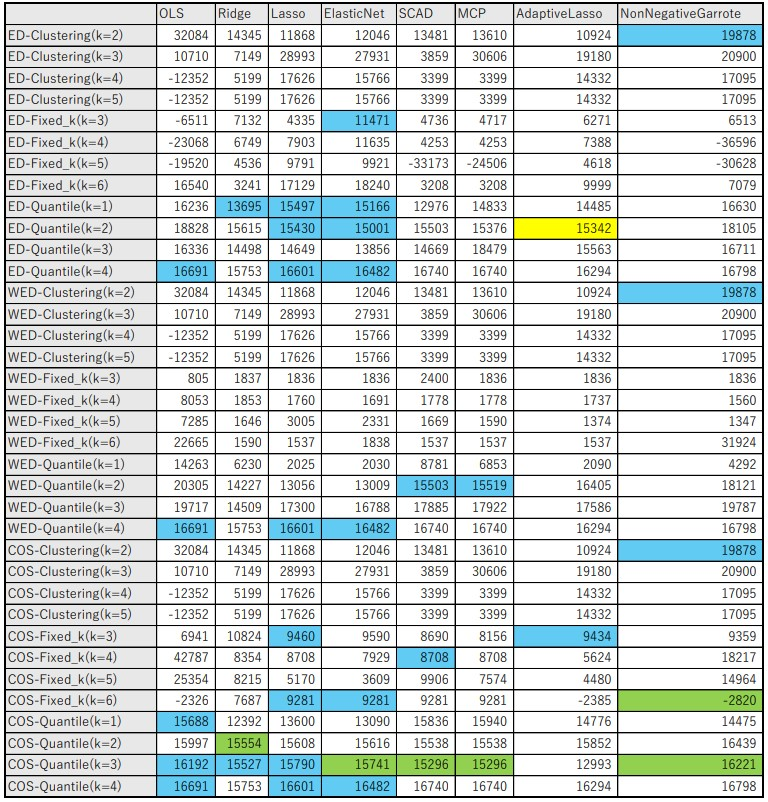
\includegraphics[width=120mm]{figure/fig/estDf_color.jpg}
  \captionsetup{labelformat=empty} % 図番号を非表示に設定
  \caption{\Fdualcaption{Colored ``Predicted Effort for New Project" Report.}{精度が高い手法の予測値}}
  \label{fig:estColor}
\end{figure}

% 第5章
\clearpage
\pagestyle{plain}
\section{結論と今後の展望}\label{sec:5}
本研究ではソフトウェア開発における開発工数予測システムの開発・改良を行った.
SDepT v2.0.0は前処理における複数手法の実装や,回帰手法の多様化により,多様化したソフトウェア開発により柔軟に対応できるツールとなった.また,ユーザーインターフェースに異なる2種類の画面を用意することで,専門的な知識を要せずに操作できることと,専門的な知識により高度な設定ができること,2つの面からユーザーフレンドリーを実現した.

一方で,Ahmedら\cite{Ahmed2022}によると,アナロジーベースの工数予測と比較して,Ahmedらが提案したブロックチェーンベースの工数予測の方が精度が優れていた.
そのため,他の手法と比較した際のアナロジーベースの予測手法の優位性について検討する必要がある.
Tibshiraniら\cite{Tibshirani2000}は,データに対して適切なクラスタ数を推定することができるギャップ統計法を提案しており,クラスタリングによって類似プロジェクトの選定をする際に,ユーザーが$k$の値を指定せずとも常に最適なクラスタ数での予測結果を提供できる可能性がある.
また,データセットの規模によって処理時間も増大するため,並列処理を用いて処理時間を削減する必要がある.
今後は,上記の課題を解決することに加え,最終的にはオープンソース化を予定している.

% tmp
% \clearpage
% \pagestyle{plain}
% \input{sections/}

% 謝辞
\clearpage
\pagestyle{plain}
\section*{謝辞}
\addcontentsline{toc}{section}{謝辞}
ここに謝辞を書く

% 参考文献
\addcontentsline{toc}{section}{参考文献}
\clearpage
\pagestyle{plain}
\bibliographystyle{jIEEEtran}
\bibliography{bibliography/references.bib}

% 付録
\clearpage
\appendix
\section{システム構成図の詳細}
\ref{sec:3}の図\ref{fig:systemarch}のシステム構成図に,各工程にて渡される変数名を追記したものを図\ref{fig:systemarch_detail}に示す.

\begin{figure}[ht]
  \centering
  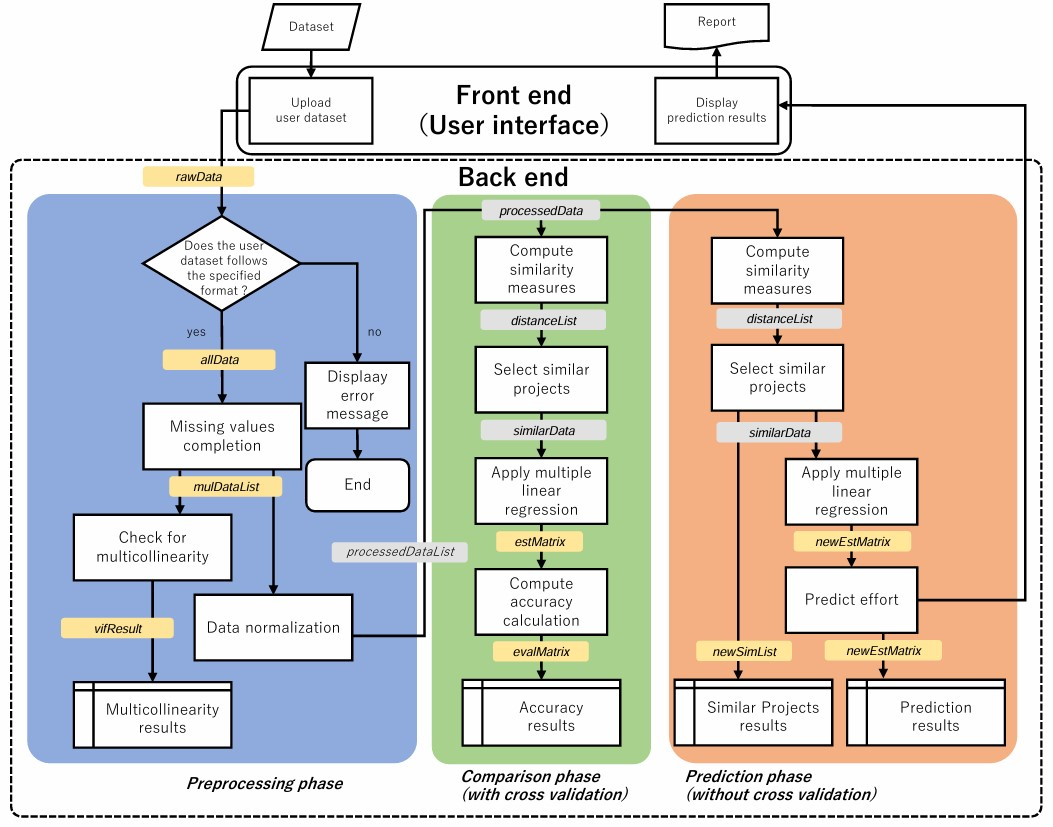
\includegraphics[width=120mm]{figure/fig/SystemArch_detail_20241123.jpg}
  \captionsetup{labelformat=empty} % 図番号を非表示に設定
  \caption{\Fdualcaption{System Architecture of SDepT v2.0.0.(detail)}{SDepT v2.0.0 システム構成図詳細版.}}
  \label{fig:systemarch_detail}
\end{figure}
%\begin{table*}[ht]
  \centering
  \captionsetup{labelformat=empty} % 図番号を非表示に設定
  \caption{\Tdualcaption{Preprocess.}{前処理.}}
  \label{table:preprocess}
  \resizebox{\textwidth}{!}{
    \begin{tabular}{|l|c|c|c|}
      \hline
      ~ & SDepT v1.0.0 & Huangら & SDepT v2.0.0 \\ \hline
      %%%%%%%%欠損値補完手法%%%%%%%%
      \multirow{4}{*}{欠損値補完} & z-score法 & z-score法 & z-score法 \\
       &  & MinMax[0, 1] & MinMax[0, 1] \\
       &  & MinMax[0, 1] & MinMax[-1, 1] \\
       &  &  & BoxCox法 \\ \hline
      %%%%%%%%正規化手法%%%%%%%%
      \multirow{4}{*}{正規化} & 中央値補完 & 平均/最頻値補完 & 中央値補完 \\
       &  & $k$最近傍補完 & 平均値補完 \\
       &  &  & 最頻値補完 \\
       &  &  & $k$最近傍補完 \\ \hline
      %%%%%%%%特徴選択手法%%%%%%%%
      \multirow{4}{*}{特徴選択} & 多重共線性の確認のみ & Null & 多重共線性の確認のみ \\
       &  & SFS\_SBS(逐次選択方式の組み合わせ) &  \\
       &  & MI(相互情報量)ベースの重み付け &  \\
       &  & GA(遺伝的アルゴリズム) &  \\ \hline
      %%%%%%%%使用データセット%%%%%%%%
      \multirow{6}{*}{使用データセット} & SDepT v1.0.0 & Huangら & SDepT v2.0.0 \\
      & SDepT v1.0.0 & Huangら & SDepT v2.0.0 \\
      & SDepT v1.0.0 & Huangら & SDepT v2.0.0 \\
      & SDepT v1.0.0 & Huangら & SDepT v2.0.0 \\
      & SDepT v1.0.0 & Huangら & SDepT v2.0.0 \\
      & SDepT v1.0.0 & Huangら & SDepT v2.0.0 \\ \hline
    \end{tabular}
  }
\end{table*}


\clearpage
\section{使用データセット及び実行結果}
\subsection{使用データセット}
本節では,本研究で用いたデータセットを紹介する.
\subsubsection{データセット1}
Desharnaisデータセット\cite{Desharnais89}(表\ref{table:DesharnaisDataset})は,1980年代のカナダのソフトウェア開発会社のプロジェクトデータが記録されており,81件の過去のプロジェクトデータと11のプロジェクト特性(チームの経験年数(TeamExp in years),開発年度(YearEnd),マネージャーの経験年数(ManageExp in years),開発年数(Length),トランザクション数(Transactions),エンティティ数(Entities),調整済みファンクションポイント(PointsAdjust),調整係数(Envergure),未調整ファンクションポイント(PointsNonAdjust),開発言語(Language),開発工数(Effort))が含まれている.

\subsubsection{データセット2}
Kitchenhamデータセット\cite{Kitchenham2002}(表\ref{table:KitchenhamDataset})はKitchenhamらが2002年から公開しているデータセットであり,あるソフトウェア開発企業のプロジェクトデータが記録されている.データセットには145件の過去プロジェクトデータと5つのプロジェクト特性(顧客番号(Clientcode),開発期間(Actualduration(Days)),調整済みファンクションポイント(Adjustedfunctionpoints),初期見積もり値(First estimate in Hour),開発工数(Actualeffort(Hours)))が含まれている.

\begin{table*}[ht]
  \centering
  \captionsetup{labelformat=empty} % 図番号を非表示に設定
  \caption{\Tdualcaption{Kitchenham Dataset of Software Development.}{Kitchenhamデータセット.}}
  \label{table:KitchenhamDataset}
  \begin{center}
    \resizebox{\textwidth}{!}{
      \begin{tabular}{|c|c|c|c|c|c|}
        \hline
        Project & Clientcode & Actualduration(Days) & Adjustedfunctionpoints & Firstestimate(Hours) & Actualeffort(Hours) \\ \hline \hline
        1 & 1 & 107 & 101.65 & 495 & 485 \\ \hline
        2 & 1 & 144 & 57.12 & 1365 & 990\\ \hline
        3 & 1 & 604 & 1010.88 & 8244 & 13635 \\ \hline
        \vdots & \vdots & \vdots & \vdots & \vdots & \vdots \\ \hline
        144 & 6 & 1560 & 1002.76 & 1039 & 104 \\ \hline
        145 & 2 & 92 & 551.88 & 1393 & 887 \\ \hline
      \end{tabular}
    }
  \end{center}
\end{table*}

\subsubsection{データセット3~6}
その他4つのデータセットは,PROMISE Software Engineering Repository\cite{PROMISEdataset}に2004年から掲載されているNASAのSoftware defect PredictionのMetrics Data Programである.それぞれのデータセットは,PC1(表\ref{table:PC1Dataset})には1109件,CM1(表\ref{table:CM1Dataset})には498件,KC1(表\ref{table:KC1Dataset})には2109件,KC2(表\ref{table:KC2Dataset})には522件の過去プロジェクトデータが記録されており,21のプロジェクト特性(McCabe's line count of code(loc),McCabe "cyclomatic complexity"(v(g)),McCabe "essential complexity"(ev(g)),McCabe "design complexity"(iv(g)),Halstead total operators + operands(n),Halstead "volume"(v),Halstead "program length"(l),Halstead "difficulty"(d),Halstead "intelligence"(i),Halstead(b),Halstead's time estimator(t),Halstead's line count(lOCode),Halstead's count of lines of comments(lOComment),Halstead's count of blank lines(lOBlank),(lOCodeAndComment),unique operators(uniq\_Op),unique operands(uniq\_Opnd),total operators(total\_Op),total operands(total\_Opnd),of the flow graph(branchCount),Halstead "effort"(e))が含まれている.なお,\ref{Preprocess}項のデータの所定書式に従い,モジュールに含まれる報告された欠陥の有無(dfectsまたはproblems)のプロジェクト特性を除いている.

\begin{table*}[ht]
  \centering
  \captionsetup{labelformat=empty} % 図番号を非表示に設定
  \caption{\Tdualcaption{PROMISE Dataset of Software Development(PC1).}{PROMISEデータセット(PC1).}}
  \label{table:PC1Dataset}
  \begin{center}
    \resizebox{\textwidth}{!}{
      \begin{tabular}{|c|c|c|c|c|c|c|c|c|c|c|c|c|}
        \hline
        Project & loc & v(g) & ev(g) & iv(g) & n & v & l & d & i & \dots & branchCount & e \\ \hline \hline
        1 & 1.1 & 1.4 & 1.4 & 1.4 & 1.3 & 1.3 & 1.3 & 1.3 & 1.3 & \dots & 1.4 & 1.3 \\ \hline
        2 & 1 & 1 & 1 & 1 & 1 & 1 & 1 & 1 & 1 & \dots & 1 & 1 \\ \hline
        3 & 91 & 9 & 3 & 2 & 318 & 2089.21 & 0.04 & 27.68 & 75.47 & \dots & 17 & 57833.24 \\ \hline
        \vdots & \vdots & \vdots & \vdots & \vdots & \vdots & \vdots & \vdots & \vdots & \vdots & $\ddots$ & \vdots & \vdots \\ \hline
        1108 & 18 & 8 & 5 & 5 & 111 & 613.12 & 0.04 & 22.92 & 26.75 & \dots & 15 & 14050.56 \\ \hline
        1109 & 26 & 18 & 13 & 6 & 228 & 1335.62 & 0.03 & 35.81 & 37.29 & \dots & 35 & 47834.26 \\ \hline
      \end{tabular}
    }
  \end{center}
\end{table*}

\begin{table*}[ht]
  \centering
  \captionsetup{labelformat=empty} % 図番号を非表示に設定
  \caption{\Tdualcaption{PROMISE Dataset of Software Development(CM1).}{PROMISEデータセット(CM1).}}
  \label{table:CM1Dataset}
  \begin{center}
    \resizebox{\textwidth}{!}{
      \begin{tabular}{|c|c|c|c|c|c|c|c|c|c|c|c|c|}
        \hline
        Project & loc & v(g) & ev(g) & iv(g) & n & v & l & d & i & \dots & branchCount & e \\ \hline \hline
        1 & 1.1 & 1.4 & 1.4 & 1.4 & 1.3 & 1.3 & 1.3 & 1.3 & 1.3 & \dots & 1.4 & 1.3 \\ \hline
        2 & 1 & 1 & 1 & 1 & 1 & 1 & 1 & 1 & 1 & \dots & 1 & 1 \\ \hline
        3 & 24 & 5 & 1 & 3 & 63 & 309.13 & 0.11 & 9.5 & 32.54 & \dots & 9 & 2936.77 \\ \hline
        \vdots & \vdots & \vdots & \vdots & \vdots & \vdots & \vdots & \vdots & \vdots & \vdots & $\ddots$ & \vdots & \vdots \\ \hline
        497 & 10 & 2 & 1 & 1 & 32 & 150.41 & 0.15 & 6.5 & 23.14 & \dots & 3 & 977.69 \\ \hline
        498 & 28 & 6 & 5 & 5 & 104 & 564.33 & 0.06 & 16.09 & 35.08 & \dots & 11 & 9078.38 \\ \hline
      \end{tabular}
    }
  \end{center}
\end{table*}

\begin{table*}[ht]
  \centering
  \captionsetup{labelformat=empty} % 図番号を非表示に設定
  \caption{\Tdualcaption{PROMISE Dataset of Software Development(KC1).}{PROMISEデータセット(KC1).}}
  \label{table:KC1Dataset}
  \begin{center}
    \resizebox{\textwidth}{!}{
      \begin{tabular}{|c|c|c|c|c|c|c|c|c|c|c|c|c|}
        \hline
        Project & loc & v(g) & ev(g) & iv(g) & n & v & l & d & i & \dots & branchCount & e \\ \hline \hline
        1 & 1.1 & 1.4 & 1.4 & 1.4 & 1.3 & 1.3 & 1.3 & 1.3 & 1.3 & \dots & 1.4 & 1.3 \\ \hline
        2 & 1 & 1 & 1 & 1 & 1 & 1 & 1 & 1 & 1 & \dots & 1 & 1 \\ \hline
        3 & 83 & 11 & 1 & 11 & 171 & 927.89 & 0.04 & 23.04 & 40.27 & \dots & 21 & 21378.61 \\ \hline
        \vdots & \vdots & \vdots & \vdots & \vdots & \vdots & \vdots & \vdots & \vdots & \vdots & $\ddots$ & \vdots & \vdots \\ \hline
        2108 & 13 & 1 & 1 & 1 & 17 & 60.94 & 0.25 & 4 & 15.24 & \dots & 1 & 243.78 \\ \hline
        2109 & 11 & 2 & 1 & 2 & 27 & 102.8 & 0.17 & 6 & 17.13 & \dots & 3 & 616.79 \\ \hline
      \end{tabular}
    }
  \end{center}
\end{table*}

\begin{table*}[ht]
  \centering
  \captionsetup{labelformat=empty} % 図番号を非表示に設定
  \caption{\Tdualcaption{PROMISE Dataset of Software Development(KC2).}{PROMISEデータセット(KC2).}}
  \label{table:KC2Dataset}
  \begin{center}
    \resizebox{\textwidth}{!}{
      \begin{tabular}{|c|c|c|c|c|c|c|c|c|c|c|c|c|}
        \hline
        Project & loc & v(g) & ev(g) & iv(g) & n & v & l & d & i & \dots & branchCount & e \\ \hline \hline
        1 & 1.1 & 1.4 & 1.4 & 1.4 & 1.3 & 1.3 & 1.3 & 1.3 & 1.3 & \dots & 1.4 & 1.3 \\ \hline
        2 & 1 & 1 & 1 & 1 & 1 & 1 & 1 & 1 & 1 & \dots & 1 & 1 \\ \hline
        3 & 415 & 59 & 50 & 51 & 1159 & 8411.31 & 0.01 & 103.53 & 81.24 & \dots & 106 & 870848.58 \\ \hline
        \vdots & \vdots & \vdots & \vdots & \vdots & \vdots & \vdots & \vdots & \vdots & \vdots & $\ddots$ & \vdots & \vdots \\ \hline
        521 & 4 & 1 & 1 & 1 & 5 & 11.61 & 0.67 & 1.5 & 7.74 & \dots & 1 & 17.41 \\ \hline
        522 & 3 & 1 & 1 & 1 & 1 & 0 & 0 & 0 & 0 & \dots & 1 & 0 \\ \hline
      \end{tabular}
    }
  \end{center}
\end{table*}

\subsection{実行結果}
\subsubsection{データセット1}

\subsubsection{データセット2}

\subsubsection{データセット3}

\subsubsection{データセット4}


\clearpage
\section{多重共線性と回帰手法における考察}\label{sec:C}
この部分は\ref{sec:4}の考察に入れる方向で考え中なので\ref{sec:C}はなくなる可能性大.

\end{document}